%%%%%%%%%%%%%%%%%%%%%%%%%%%%%%%%%%%%%%%%%%%%%%%%%%%%%%%%%%%%%%%%%%%%%%%%%%%%%%%%
%                                                                              %
%   KUIP  - Reference Manual -- LaTeX Source                                   %
%   Modified for PAW. Comes from:   Chapter 2: User Interface (KUIP manual)    %
%                                                                              %
%   Author: Alfred Nathaniel  CN/ASD                                           %
%   Editor: Michel Goossens   IT/ASD                                           %
%   Mods:   30 July 1998 Olivier Couet                                         %
%                                                                              %
%%%%%%%%%%%%%%%%%%%%%%%%%%%%%%%%%%%%%%%%%%%%%%%%%%%%%%%%%%%%%%%%%%%%%%%%%%%%%%%%

\def\PROMPT{\texttt{PAW >}}


--------------------------------------------------------------------
%
\section{Command line syntax\label{sec-command-line-syntax}}

The general syntax of a \emph{command line} is a \emph{command path}
optionally followed by an \emph{argument list}.
The command path and the arguments have to be separated from each other by one
or more space characters.
Therefore arguments containing spaces or other special characters have
to be quoted.

In the following we want to use an appropriate formalism to describe the
syntax rules.
The notation will be introduced step by step as needed.
The verbal explanation given above can be written as:

\indent\indent\begin{tabular}{rcl}
\textsl{command-line}
&\texttt{::=}&\textsl{command-path \quad \lcb\ argument \rcb}
\end{tabular}

The \textsl{slanted} symbols are non-terminal, i.e.\ they are composed
of other terminal or non-terminal symbols.  The definition of a
non-terminal symbol is denoted by ``\textbf{::=}''.  Symbols enclosed
in braces (``\texttt{\lcb...\rcb}'') are optional and they can appear
  zero or more times.

%
%---------------------------------------------------------------------------
%
\subsection{Command structure}

The set of commands is structured as an (inverted) tree as shown in
figure~\ref{FIG7}.
 
\begin{figure}[h]
\centering\includegraphics[width=.8\linewidth]{tree.eps}
\caption{Example of the PAW command tree structure}
\label{FIG7}
\end{figure}
 
This structure is comparable to a Unix file system.  The command set
can be dynamically extended by linking new commands or menus into the
tree.  Compared to a flat list structure the tree allows a cleaner
representation through menus, especially when the command set is
large.  \PAW{} has more than 200~commands.  It would be hard to
visualize such a number of command in a single graphics menu.

%
%---------------------------------------------------------------------------
%
\subsubsection{Abbreviations}

A command path consists of a menu path and a command name.
The menu path itself consists of a list of menu names up to an
arbitrarily deep level of sub-menus.

\indent\indent\begin{tabular}{rcl}
\textsl{command-path}
&\texttt{::=}&\textsl{\lsb menu-path\texttt{/\rsb}command-name} 
\\
\textsl{menu-path} 
&\texttt{::=}&
\textsl{\texttt{[/]}menu-name\texttt{\lcb/}menu-name\rcb}
\end{tabular}

Here we introduced two more notations.
Symbols in teletype mode (``\texttt{/}'') are literals, i.e.\
the menu and command names have to be separated by a slash character.
Symbols enclosed in brackets (``\texttt{[...]}'') are optional which can
appear zero or one times.

These syntax rules already show that a command path may be abbreviated by
omitting part of the leading menu path.
For example, if the complete command path is
\begin{alltt}
/MENU/SUBMENU/COMMAND
\end{alltt}
valid abbreviations are
\begin{alltt}
MENU/SUBMENU/COMMAND
SUBMENU/COMMAND
COMMAND
\end{alltt}
but \textbf{not} ``\texttt{MENU/COMMAND}'' or
``\texttt{/SUBMENU/COMMAND}''.
Note that the command name matching is case-insensitive, i.e.\ the
following are all valid possibilities:
\begin{alltt}
COMMAND
command
Command
\end{alltt}

Furthermore, menu and command names may be abbreviated by omitting
trailing parts, i.e.\
\begin{alltt}
SUB/COMMAND
COMMA
/M/S/C
\end{alltt}
are also valid abbreviations.

The shortest unambiguous abbreviation for any command is not fixed
but depends on the whole command set.
PAW lists all possible ambiguities if a given abbreviation has no
unique match:

\begin{alltt}
PAW > \underline{LIST}
 *** Ambiguous command list. Possible commands are :

 /KUIP/ALIAS/LIST
 /MACRO/LIST
 /VECTOR/LIST
 /HISTOGRAM/LIST
 /NTUPLE/LIST
 /PICTURE/LIST
\end{alltt}

\paragraph{Changing the root menu}

The command \texttt{SET/ROOT} defines the menu from which the search for
command name starts. 
It is not quite comparable to the Unix \texttt{cd} or VMS 
\texttt{SET DEFAULT} command.
If no matching command is found going downwards from the
\texttt{SET/ROOT} menu a second attempt is made starting off at the top
menu ``\texttt{/}''.

\paragraph{Disabling commands}

The command \Cind{SET/VISIBILITY} allows to disable/enable individual commands.
\index{command!visibility}
Disabled commands cannot be executed and they do not contribute to
name ambiguities.
However, the \Cind{HELP} information is still available.
Note that the \Cind{VISIBILITY} command can disable itself which makes
it impossible to re-enable any command.


\paragraph{Automatic macro execution}

The command \Cind{MACRO/DEFAULT} implements two facilities.
First it allows to define a directory search path used by the
\Cind{EXEC} command for locating \texttt{.kumac} macro files.
Second it controls the implicit interpretation of the command name token as a
possible macro filename:
\begin{DLtt}{-AutoReverse}
\item[\texttt{-Command}]
This is the default setting which does not try to interpreted
\texttt{cmd} as macro name.
\item[\texttt{-Auto}]
If the search path contains a file \texttt{cmd.kumac} it is executed,
i.e.\ the actual command becomes ``\texttt{EXEC cmd}'', otherwise the
search for a command named \texttt{cmd} starts.
\item[\texttt{-AutoReverse}]
If \texttt{cmd} is either not a command name or ambiguous and a file
\texttt{cmd.kumac} exists the command is transformed into 
``\texttt{EXEC cmd}''.
\end{DLtt}


\paragraph{Command template\label{para-set-command}}

The command \Cind{SET/COMMAND} allows to define a template which is
used whenever the command token does not match any command name.
The template can contain ``\verb!$1!'',\dots, ``\verb!$9!'' which are
substituted with the \textsl{n}'th token from the original command line,
or ``\verb!$*!'' which is replaced by the complete line.
For example, PAW can be turned into a calculator by
\begin{alltt}
\PROMPT{} \underline{SET/COMMAND 'mess $sigma($*)'}
\PROMPT{} \underline{17+2*5}
 27
\end{alltt}

``\verb!SET/COMMAND 'EXEC $*'!'' has almost the same effect as 
``\verb!DEFAULT -AutoReverse!'' but these are two distinct facilities
which can be active simultaneously.
The difference is that for \texttt{SET/COMMAND} the token in the command
name position must not match any command.
If does not apply if the token is an ambiguous command name.

Both \texttt{Auto/AutoReverse} and \texttt{SET/COMMAND} logic are ignored
during the execution of macro scripts.


%
%---------------------------------------------------------------------------
%
\subsection{Arguments}

Most commands have \emph{parameters} for which the user is expected to
supply \emph{argument values}.
Parameters are either \emph{mandatory} or \emph{optional}.
Mandatory arguments which are not specified on the command line are
prompted for.
If optional arguments are omitted a default value is used instead.

Mandatory parameters always precede the optional parameters.
The command \Cind{USAGE} allows to see the number of parameters for a command:
\begin{alltt}
\PROMPT{} \underline{usage manual}

 * KUIP/MANUAL ITEM [ OUTPUT OPTION ]
\end{alltt}
The optional parameters are enclosed in square brackets.
The default values can be seen from the help text for a command.
The \texttt{STYLE} command shown in figure~\ref{fig-help-style} 
has only optional arguments.
The corresponding default values are indicated in the help information
as ``\texttt{D=}\textsl{value}''.

\begin{figure}
\begin{alltt}
\PROMPT{} \underline{HELP STYLE}

 * KUIP/SET_SHOW/STYLE [ OPTION SGYLEN SGSIZE SGYSPA SGBORD WKTYPE ]

   OPTION     C 'Option' D='?'
   SGYLEN     R 'max Y LENgth of each menu item box' D=0.025 R=0.005:0.25
   SGSIZE     R 'space available for the application' D=0.8 R=0:0.90
   SGYSPA     R 'max Y length of space between menus' D=0.02 R=-0.5:0.50
   SGBORD     R 'X or Y border for menus' D=0.015 R=0:0.25
   WKTYPE     I 'Graphics workstation type' D=0

   Possible OPTION values are:

    ?   show current style
    C   Command line : select Command line input
    AN  Menu with Numbers : select general Alpha menu (with Numbers)
    AL  Menu with Letters : select general Alpha menu (with Letters)
\end{alltt}
\caption{Parameter types, default values, and range limits
\label{fig-help-style}}
\end{figure}

Mandatory parameters may also have a default value which is used if
the prompt is acknowledged by simple hitting the \texttt{RETURN}-key.
Otherwise the proposed default is the value used in the previous
command execution.

The \texttt{STYLE} command also shows that there are three different
kind of parameters:
character values indicated by ``\texttt{C}'' after the parameter
name, real values (``\texttt{R}'') and integer values
(``\texttt{I}'').

Numeric (real or integer) parameters may be restricted in the range of
acceptable values.
In the help text this is indicated as
``\texttt{R=\textsl{lower}:\textsl{upper}}. 
If the argument value is outside the range PAW  prompts the user to
enter an acceptable value before the command can be executed.
The lower or upper range value may be missing to indicate an unlimited
range in one direction.
Instead of a simple numeric value the argument may also be an expression.

For both numeric and character parameters the range may also be given
as a comma-separated list of values. 
PAW will accept an argument only if it matches one of
the values in the list.

In general the arguments given on the command line are assigned to the
command parameters from left to right but there are also ways to
change the order.
In our syntax notation, using ``\texttt{|}'' to indicate possible
alternatives, we can write:

\begin{tabular}{rclclclclclcl}
\textsl{argument}
&\texttt{::=}&
\textsl{value} 
&\verbar&
\texttt{!} 
&\verbar&
\texttt{!!} 
&\verbar&
\textsl{name\texttt{=}value} 
&\verbar&
\textsl{\texttt{-}value} 
\end{tabular}

An argument given as a simple value is assigned to the next parameter
expected. 
The special values ``\texttt{!}'' and ``\texttt{!!}'' are templates
for the default value and the value from the previous command
execution, respectively.

\subsubsection{Named arguments\label{sec-named-arguments}}

The form ``\textsl{name\texttt{=}value}'' allows to invert the
argument order or to skip a list of optional parameters for which
the default values should be used.
For example,
\begin{alltt}
STYLE G SGBORD=0.1
\end{alltt}
is equivalent to 
\begin{alltt}
STYLE G ! ! ! 0.1
\end{alltt}
A simple argument following a named argument is assigned to the
parameter following the named parameter, i.e.\
\begin{alltt}
STYLE G SGBORD=0.1 1
\end{alltt}
is equivalent to 
\begin{alltt}
STYLE G ! ! ! SGBORD=0.1 WKTYPE=1
\end{alltt}

Parameter names are case-insensitive but in general they may not be
abbreviated. 
In the help text the abbreviat level is indicated by a ``\texttt{*}'' inside 
the parameter name.
For example, if the parameter name is shown as
\begin{alltt}
LIB*RARY
\end{alltt}
the acceptable abbreviations are ``\texttt{LIB=}'',
``\texttt{LIBR=}'', ``\texttt{LIBRA=}'', ``\texttt{LIBRAR=}'', and
``\texttt{LIBRARY=}''.

PAW does not insist that an argument of the form
``\textsl{name\texttt{=}value}'' matches one of the parameter names. 
The argument including the ``\textsl{name\texttt{=}}'' part is simply
assigned to the next parameter expected.


\subsubsection{Option arguments}

The last alternative ``\texttt{-}\textsl{value}'' to specify an
argument applies only to \textsl{option} parameters.
(Note the distinction between \emph{option} and \emph{optional}.
Option parameters are usually but not necessarily optional.)
In the help text option parameters are tagged by the list of possible
values (figure~\ref{fig-help-manual}).
Frequently these parameters are named ``\texttt{OPTION}'' or
``\texttt{CHOPT}''. 

\begin{figure}
\begin{alltt}
PAW > \underline{HELP MANUAL}

 * KUIP/MANUAL ITEM [ OUTPUT OPTION ]

   ITEM       C 'Command or menu path'
   OUTPUT     C 'Output file name' D=' '
   OPTION     C 'Text formatting system' D=' '

   Possible OPTION values are:

   ' '     plain text : plain text format
    LATEX  LaTeX format (encapsulated)
    TEX    LaTeX format (without header)
\end{alltt}
\caption{Example for option parameters
\label{fig-help-manual}}
\end{figure}

The ``\texttt{-}\textsl{value}'' form allows to specify option
arguments out of order, emulating the Unix style of options preceded
other command arguments.
For example,
\begin{alltt}
MANUAL -LATEX /KUIP
\end{alltt}
is equivalent to 
\begin{alltt}
MANUAL /KUIP OPTION=LATEX
\end{alltt}
Note that this is \textbf{not} equivalent to 
``\texttt{MANUAL OPTION=LATEX /KUIP}''.
Unlike to the ``\texttt{-}\textsl{value}'' form subsequent simple
arguments are still assigned to the next parameter expected, not to
the one following the option parameter itself.

Since a leading ``\texttt{-}'' can be part of a valid (non-option)
argument the value is checked against a set of rules before it is
actually interpreted as an option assignment.

The option argument can be a concatenation of several of the allowed
option values.
PAW checks that the argument string is exclusively constructed from
valid option values.
This check is done by removing matches of option values from the
argument string, starting with the longest option values first.
For example, with the definition
\begin{alltt}
   Possible OPTION values are:
    AB
    ABC
    CD
\end{alltt}
the argument ``\texttt{-ABCD}'' is not interpreted as option
assignment because after removing the longest match ``\texttt{ABC}''
the remainder ``D'' is not anymore a valid option value.
(This case would have to be written as ``\texttt{-CDAB}''.

%
%---------------------------------------------------------------------------
%
\subsubsection{Argument values}

Since in command line blanks are used to separate the command name and the 
individual arguments string values containing blanks have to be quoted. The 
rules are the same as used by Fortran: the quote character is the apostrophe
``\texttt{'}'', and apostroph inside a quoted string have to be duplicated:

\begin{alltt}
MESS 'Hello world'
MESS 'Do or don''t'
\end{alltt}

Note that the \Cind{MESSAGE} command has only a single parameter:
\begin{alltt}
 * KUIP/MESSAGE [ STRING ]

   STRING     C 'Message string' D=' '
...
\end{alltt}
Nevertheless, in most cases quoting the message string is not necessary. If the 
command line contains more arguments than there are parameters the additional 
values are concatenated to the argument for the last parameter. In the 
concatenation each value is separated by a (single) blank character, i.e.\ 
the commands

\begin{alltt}
MESS 'Hello World'
MESS  Hello World
MESS  Hello       World
\end{alltt}
yield all the same output. Therefore the message text only needs quoting if the 
words should be separated by more than one space character.

Quoting inhibits the interpretation of the enclosed string as special argument
values. Printing an exclamation mark as message text has to written as

\begin{alltt}
MESS '!'
\end{alltt}

because ``\texttt{MESS !}'' would mean to take the default value for the 
parameter \Pind{STRING} and yield an empty line only.

Another instance is if an argument of the form ``\textsl{name\texttt{=}value}'' 
should be taken literally. For example, the command line

\begin{alltt}
EXEC mac foo=bar
\end{alltt}

initializes the macro variable ``\texttt{foo}'' to the value ``\texttt{bar}''. 
However, if the intention is to pass the string ``\texttt{foo=bar}'' as 
argument to the macro quotes must be used:

\begin{alltt}
EXEC mac 'foo=bar'
\end{alltt}

In addition, some commands, e.g.\

\begin{alltt}
 * NTUPLE/PLOT IDN [ UWFUNC NEVENT IFIRST NUPD OPTION IDH ]
\end{alltt}

use the form ``\textsl{name\texttt{=}value}'' for equality tests in the cut 
expression \Pind{UWFUNC}.  For example, the command

\begin{alltt}
NT/PLOT 10.energy year=1998
\end{alltt}

selects all event for which the Ntuple column \texttt{YEAR} has the value 
\texttt{1998}. Any name clash between the Ntuple column and one of the command
parameters requires quoting. If the column was called \texttt{NUPD} instead of
\texttt{YEAR} the command would have to be written as

\begin{alltt}
NT/PLOT 10.energy 'nupd=1998'
\end{alltt}

or alternatively as ``\texttt{NT/PLOT 10.energy UWFUNC=nupd=1998}''.

Finally, quoted strings are also exempted from any substitutions of aliases, 
\Key{system function}s, and \Key{macro variable}s. For example,

\begin{alltt}
MESS 'foo'
\end{alltt}
always prints ``\texttt{foo}'' while
\begin{alltt}
MESS foo
\end{alltt}

can result in ``\texttt{bar}'' if preceded by the command
``\texttt{ALIAS/CREATE foo bar}''. Since square brackets denote macro variable 
substitution and system functions names start with a dollar-sign it is 
especially recommended to quote VMS file specifications.

The operator ``\texttt{//}'' allows to concatenate several parts to a single 
argument value. Unquoted strings on either side of the concatenation operator 
are implicitly treated as literals unless they are subject to a substitution, 
i.e.\ the command lines

\begin{alltt}
MESS 'abc'//'def'
MESS 'abc'//def
MESS abc//'def'
MESS abc//def
MESS abcdef
MESS 'a'//'b'//'c'//'d'//'e'//'f'
\end{alltt}

are all equivalent (provided that \texttt{abc} and \texttt{def} are not defined 
as aliases). The character sequence ``\texttt{//}'' at the beginning or end of 
an argument is taken literally, e.g.\ in

\begin{alltt}
CD //LUN2//1
\end{alltt}

the command receives the value ``\texttt{//LUN21}''.


\subsection{More on command lines}

The command line syntax allows to write several commands in one line
and also to extend commands with long argument
lists over several lines.


\subsubsection{Multiple commands on a single line\label{sec-mult-cmd}}

An input line presented to the PAW command processor may contain
several commands separated by ``\texttt{;}''.
The commands are executed sequentially as if they were on separate
lines:
\begin{alltt}
MESS Hello world!; MESS How are you?
\end{alltt}
is equivalent to
\begin{alltt}
MESS Hello world!
MESS How are you?
\end{alltt}
Note that the text following the semicolon will not be used to satisfy
any prompts emitted by the preceding command, 
e.g.\ ``\texttt{usage; manual}'' will not behave as 
``\texttt{usage manual}''.

The semicolon is \textbf{not} interpreted as line
separator if it is immediately followed by a digit or one of the
characters
\begin{alltt}
  +  - *  ?  [
\end{alltt}
For example, issuing a VMS command with a file version number such as
\begin{alltt}
SHELL delete *.tmp;*
\end{alltt}
does not require quoting.
Note that this exception rule applies independently of the operating
system.
In order to avoid surprises we recommend to put always at least one
blank after a semicolon intended to be a line separator.

Each command execution returns a status code which is zero for success
and non-zero for failure.
The sequences ``\texttt{;\&}'' and ``\texttt{;!}'' allow to execute
the remaining part of an input line depending on the status code of
the preceding command.
With
\begin{alltt}
cmd1 ;& cmd2 ; cmd3
\end{alltt}
the commands \Cind{cmd2} and \Cind{cmd3} are only executed if
\Cind{cmd1} succeeded while with
\begin{alltt}
cmd1 ;! cmd2 ; cmd3
\end{alltt}
the remaining commands are only executed if the first one failed.
Note that the two characters must follow each other immediately
without intervening blank.

In some commands, for example \Cind{HISTO/PLOT}, one of the parameters
is marked in the help text with the attribute ``\texttt{Loop}''.
If the corresponding argument is a comma-separated list of values
PAW implicitly repeats the command for each value in the list
individually: 
\begin{alltt}
HISTO/PLOT 10,20,30
\end{alltt}
is equivalent to
\begin{alltt}
HISTO/PLOT 10
HISTO/PLOT 20
HISTO/PLOT 30
\end{alltt}
Note that ``\texttt{,}'' inside parentheses is not taken as value
separator, i.e.\
\begin{alltt}
HISTO/PLOT 10(1:25,1:25)
\end{alltt}
executes a single command.


\subsubsection{Single commands on multiple lines}

For commands with very long argument lists it can become necessary to
continue it on the next line.
An input line ending with an ``\verb!_!'' character is joined with
the following line.

In the concatenation the underscore itself and all but one of the
leading blanks from the next line are removed.
Blanks preceding the underscore are left intact.
For example,
\begin{alltt}
ME_
SS _
'Hello_
       world'
\end{alltt}
is an extravagant way of writing
\begin{alltt}
MESS 'Hello world'
\end{alltt}
Note that the interpretation of ``\verb!_!'' as line continuation
cannot be escaped.
If the command line should really end with an underscore the last
argument must be quoted.

%
%---------------------------------------------------------------------------
%
\subsubsection{Recalling previous commands}

The command lines types during a session are written into a history file.
By default the file is called \texttt{last.kumac} and is updated every
25~commands.
The commands \Cind{LAST} and \Cind{RECORDING} allow to change the file
name and the frequency.
At the start of a new session the existing file is renamed into
\texttt{last.kumacold} (except on VMS) before the new \texttt{last.kumac} is created.
Comment lines indicate the date and time at which the sessions were
started and stopped. 

\begin{table}\centering
\begin{tabular}{|l|p{.85\textwidth}|}
\hline
\texttt{{\Circ}A/{\Circ}E  } & Move cursor to beginning/end of the line. \\
\texttt{{\Circ}F/{\Circ}B  } & Move cursor forward/backward one character. \\
\texttt{{\Circ}D     } & Delete the character under the cursor. \\
\texttt{{\Circ}H, DEL} & Delete the character to the left of the cursor. \\
\texttt{{\Circ}K     } & Kill from the cursor to the end of line. \\
\texttt{{\Circ}L     } & Redraw current line. \\
\texttt{{\Circ}O     } & Toggle overwrite/insert mode. Text added in overwrite mode
               (including yanks) overwrites existing text, while insert mode
               does not overwrite. \\
\texttt{{\Circ}P/{\Circ}N  } & Move to previous/next item on history list. \\
\texttt{{\Circ}R/{\Circ}S  } & Perform incremental reverse/forward search for string on
               the history list.  Typing normal characters adds to the
               current search string and searches for a match.  Typing
               \verb!^R/^S! marks the start of a new search, and
moves on to 
               the next match.  Typing \verb!^H! or \texttt{DEL} deletes the last
               character from the search string, and searches from the
               starting location of the last search.
               Therefore, repeated \texttt{DEL}'s appear to unwind to the match
               nearest the point at which the last \verb!^R! or
\texttt{{\Circ}S} was typed. 
               If \texttt{DEL} is repeated until the search string is empty the
               search location begins from the start of the history
               list. Typing \texttt{ESC} or any other editing character accepts
               the current match and loads it into the buffer,
               terminating the search. \\
\texttt{{\Circ}T     } & Toggle the characters under and to the left of the cursor. \\
\texttt{{\Circ}U     } & Kill from the prompt to the end of line. \\
\texttt{{\Circ}Y     } & Yank previously killed text back at current location.
               Note that this will overwrite or insert, depending on
               the current mode. \\
\texttt{TAB    } & By default adds spaces to buffer to get to next \texttt{TAB} stop
               (just after every 8th column). \\
\texttt{LF, CR } & Returns current buffer to the program. \\
\hline
\end{tabular}
\caption{Key-binding for recall style {\tt KSH}
\label{tab-recall-ksh}}
\end{table}

In this way the user can keep track of all commands entered in
the previous and in the current session.
The command ``\texttt{LAST -99}'' flushes the buffered lines into
\texttt{last.kumac} and envokes the editor on the file.
The user can then extract the interactively typed commands and copy
them into another \texttt{.kumac} file from which they can be
re-executed.

The command ``\texttt{LAST -\textsl{n}}'' prints the last \textsl{n}
commands entered.
On a workstation this allows to re-execute command sequences by doing
cut-and-paste operations with the mouse.

PAW provides a mechanism similar to the one found
in the Unix \texttt{csh} shell for re-executing commands:
\begin{DLtt}{12345}
\item[\texttt{!-}\textsl{n}]
executes the \textsl{n}'th last command once more. 
\item[\texttt{!!}]
is an short-cut for ``\texttt{!-1}'' re-executing the last command.
\item[\texttt{!}\textsl{n}]
re-executes the \textsl{n}'th command entered since the beginning of the
session.
\item[\texttt{!}]
prints the commands together with their numbers.
The number of lines printed depend on the recording frequency.
\item[\texttt{!}\textsl{foo}]
re-executed the latest command line starting with the string ``\textsl{foo}''.
\end{DLtt}

The command line numbering can also be seen if the prompt string
contains ``\texttt{[]}'':
\begin{alltt}
\PROMPT{} \underline{PROMPT 'Paw[] '}
Paw[2]
\end{alltt}

On Unix and VMS PAW also provides recalling and editing of command lines
for re-executing.
The command \Cind{RECALL} allows to choose between different
key-bindings:
\begin{UL}
\item
Recall style \texttt{KSH} has an Emacs-like binding
(table~\ref{tab-recall-ksh}) similar to
the one used by the \texttt{ksh} and \texttt{bash} shells.
If the terminal returns ANSI escape sequences the arrow keys can be
used instead of \verb!^B/^F/^N/^P!. 

\item
Recall style \texttt{DCL} implements the key-binding of VMS line
editing (table~\ref{tab-recall-dcl}).

\item
The style names \texttt{KSHO} and \texttt{DCLO} allow to switch to overstrike
mode instead of the default insert mode.

\item
Recall style \texttt{NONE} directs PAW to do plain reading from the
terminal input. 
\end{UL}

\begin{table}\centering
\begin{tabular}{|l|l|}
\hline
\verb!BS/^E! & Move cursor to beginning/end of the line. \\
\verb!^F/^D! & Move cursor forward/backward one character. \\
\verb!DEL!   & Delete the character to the left of the cursor. \\
\verb!^A!    & Toggle overwrite/insert mode. \\
\verb!^B!    & Move to previous item on history list. \\
\verb!^U!    & Delete from the beginning of the line to the cursor. \\
\verb!TAB!   & Move to next \texttt{TAB} stop. \\
\verb!LF,CR! & Returns current buffer to the program. \\
\hline
\end{tabular}
\caption{Key-binding for recall style {\tt DCL}
\label{tab-recall-dcl}}
\end{table}

%
%---------------------------------------------------------------------------
%
\section{Aliases}

\Key{Alias}es allow the user to define abbreviations for parts of a
command line.
There are two types of aliases,
\emph{command aliases} and \emph{argument aliases}, which differ
in the way they are recognized in a command line.
Both alias types can be defined by the \Cind{ALIAS/CREATE} command:
\begin{alltt}
 * KUIP/ALIAS/CREATE NAME VALUE [ CHOPT ]

   NAME       C 'Alias name'
   VALUE      C 'Alias value'
   CHOPT      C 'Option' D='A'

   Possible CHOPT values are:

    A  create an Argument alias
    C  create a Command alias
    N  No alias expansion of value
\end{alltt}

The alias value may be any string but the alias name can only consist
letters, digits, ``\verb!_!'', ``\texttt{-}'', ``\texttt{@}'',
and ``\verb!$!'' characters.
Command and argument aliases share the same name space. 
If a command alias with the same name as an existing argument alias is
created, the argument alias is deleted first, and vice versa.


\subsection{Argument aliases}

If an argument alias name is recognized anywhere
in the command line it is substituted by its value.
The name matching is case-insensitive and the substitution is literally,
i.e.\ without case folding or insertion of additional blanks.
The replacement is scanned for further occurrences of alias names which
in turn will be replaced as well.

The alias name must be separated from the rest of the
command line either by a blank or by one of the special characters
\begin{alltt}
  /  ,  =  :  ;  .  %  '  (  )
\end{alltt}
(not necessarily the same character on both sides).
For example, if \texttt{foo} and \texttt{bar} are alias names,
\texttt{foot} and \texttt{Bar-B-Q} are not affected.
If two alias replacements need to be concatenated the ``\texttt{//}''
operator can be used, i.e.
\begin{alltt}
ALIAS/CREATE DIR disk$user:[paw]
ALIAS/CREATE FIL file.dat
HISTO/FILE 1 DIR//FIL
\end{alltt}
translates into ``\verb!HISTO/FILE 1 disk$user:[paw]file.dat!''.
Since argument aliases are also recognized in the command position with
the definition abbreviations like \Cind{HISTO/FIL} cannot be used anymore.

Alias substitution does not take place inside quoted strings.
The \texttt{ALIAS} commands themselves are treated as a special case.
In the command line parsing they are specifically exempted from alias
translation in order to allow aliases can be deleted and redefined
without quoting.
For example,
\begin{alltt}
\PROMPT{} \underline{ALIAS/DELETE *}
\PROMPT{} \underline{ALIAS/CREATE foo bar}
\PROMPT{} \underline{ALIAS/CREATE bar BQ}
\PROMPT{} \underline{ALIAS/CREATE foo tball}
\PROMPT{} \underline{ALIAS/LIST}
 Argument aliases:
 BAR        => BQ
 FOO        => tball
 No Command aliases defined.
\end{alltt}
redefines \texttt{FOO} rather than creating a new alias name~\texttt{BQ}.
The value part, however, is subject to alias translations.
If the aliases are created in reverse order
\begin{alltt}
\PROMPT{} \underline{ALIAS/DELETE *}
\PROMPT{} \underline{ALIAS/CREATE bar BQ}
\PROMPT{} \underline{ALIAS/CREATE foo bar}
\PROMPT{} \underline{ALIAS/LIST}
 Argument aliases:
 BAR        => BQ
 FOO        => BQ
 No Command aliases defined.
\end{alltt}
the second alias is created as ``\texttt{ALIAS/CREATE foo BQ}''.
In this case quoting the alias value does not avoid the translation.
Writing instead
\begin{alltt}
ALIAS/CREATE foo 'bar'
\end{alltt}
will yield the same result.
Since the \texttt{ALIAS} commands bypass part of the command line parsing
the translation of the value part has to be applied by the
\Cind{ALIAS/CREATE} command itself.
At that stage the information about quoting is no longer available. 

The option ``\texttt{N}'' allows to inhibit the alias expansion in the
value.
Using this option can lead to an infinite recursion of alias
translations which will be detected only when one the alias
names involved is actually used.
\begin{alltt}
\PROMPT{} \underline{ALIAS/DELETE *}
\PROMPT{} \underline{ALIAS/CREATE foo bar}
\PROMPT{} \underline{ALIAS/CREATE -N bar foo}
\PROMPT{} \underline{ALIAS/LIST}
 Argument aliases:
 BAR        => foo
 FOO        => bar
 No Command aliases defined.
\PROMPT{} \underline{foo}
 *** Recursive command alias in foo
 *** Recursive argument alias in foo
 *** Unknown command: foo
\PROMPT{} \underline{bar}
 *** Recursive command alias in bar
 *** Recursive argument alias in bar
 *** Unknown command: bar
\end{alltt}

Alias substitution happens before the command line is split-up into
command name and arguments.
Hence, aliases can represent several arguments at once.
For example,
\begin{alltt}
ALIAS/CREATE limits '100 -1.57 1.57'
FUN1 10 sin(x) limits
\end{alltt}
is equivalent to
\begin{alltt}
FUN1 10 sin(x) 100 -1.57 1.57
\end{alltt}
The quotes in the \Cind{ALIAS/CREATE} command are necessary but they are
not part of the alias value.
If an alias value containing blanks is supposed to be treated as a
single argument four extra quotes are needed in order that
\begin{alltt}
ALIAS/CREATE htitle '''X vs. Y'''
1D 10 htitle 100 0 1
\end{alltt}
is equivalent to
\begin{alltt}
1D 10 'X vs. Y' 100 0 1
\end{alltt}

Argument aliases can lead to unexpected interpretations of command lines.
For example, a user defining
\begin{alltt}
ALIAS/CREATE e EDIT
\end{alltt}
wants ``\texttt{E}'' to be short-hand for the command \Cind{EDIT}.
However, the following consequence is probably not intended:
\begin{alltt} 
PAW > \underline{nt/plot 30.e}
 ***** Unknown name ---> EDIT
\end{alltt}

For historic reasons the default option for the \Cind{ALIAS/CREATE}
command is to define an argument alias.
However, the use of argument aliases can lead to subtle side-effects and
should therefore be restricted as much as possible. 


\subsection{Command aliases}

This problem described above does not arise if a command alias is
created instead: 
\begin{alltt}
ALIAS/CREATE -C e EDIT
\end{alltt}
Command aliases are only recognized if they appear at the beginning of a
command line (ignoring leading blanks).
Hence, there is no need to protect command arguments from inadvertent
substitutions.
Furthermore the match must be exact (ignoring case differences), i.e.
the command
\begin{alltt}
/GRAPHICS/HPLOT/ERRORS
\end{alltt}
can still be abbreviated as \Cind{HPLOT/E}.

Alias values can also represent several commands by using one of the
line separators described in section~\ref{sec-mult-cmd}, e.g.
\begin{alltt}
ALIAS/CREATE -C ciao 'MESS Hello world! ; MESS How are you?'
\end{alltt}

%
%---------------------------------------------------------------------------
%
\section{System functions}\label{sec-system-functions}
\index{function|see system function}

A set of built-in, so-called \Key{system function}s 
is provided. They allow, for example, to
inquire the current dialogue style or to manipulate strings.
The complete list of available functions can be obtained from 
``\Cind{HELP KUIP/FUNCTIONS}''.

The function name is preceded by a \verb!$!-sign.
Arguments are given as a comma separated
list of values delimited by ``\texttt{(}'' and ``\texttt{)}''.
The arguments may be expressions containing other system functions.
\index{system function!arguments}

Functions without arguments must be followed by a character which is
different from a letter, a digit, an underscore, or a colon\footnote{
Excluding the colon as separator avoids the substitution of VMS
logical name containing a dollar-sign such as in 
``\texttt{DISK\$OS:[dir]file.dat!''}}.
``\verb!$OSMOSIS!'' will not be recognized as the function
``\verb!$OS!'' followed by ``\texttt{MOSIS}''.
If that is the desired effect the concatenation operator has to be used:
``\verb!$OS//MOSIS!''. 
Note however that two functions can follow each other, e.g.\
``\verb!$OS$MACHINE!'' because the \verb!$!-sign does
not belong to the function name.
\index{system function!name separators}

Depending on the setting of the \Cind{SET/DOLLAR} command
the name following the \verb!$!-sign may also be an environment
variable\footnote{%
  On VMS there is a distinction between lowercase and uppercase names.
  Uppercase names (without the \texttt{\$}-sign) are searched for
  first in the logical name tables and then in the symbol table while
  lowercase names are searched for only in the symbol table.  The
  names \texttt{HOME}, \texttt{PATH}, \texttt{TERM}, and \texttt{USER}
  have a predefined meaning.  In order to avoid conflicts with DCL
  symbols which are merely defined as abbreviations for running
  executables and DCL procedures all values starting with a
  ``\texttt{\$}'' or ``\texttt{@}'' character are excluded from
  substitution.}.  
The replacement value for ``\verb!$!\textsl{xxx}'' is obtained 
in the following order:
\begin{OL}
\item
If \textsl{xxx} is a system function followed by the correct
number and types of arguments, replace it by its value.
\item
Otherwise if \textsl{xxx} is an argument-less system functions, replace it by
its value.
\item
Otherwise if \textsl{xxx} is a defined environment variable, replace it
by its value.
\item
Otherwise no replacement takes place.
\end{OL}


\subsection{Inquiry functions}


\subsubsection{Style inquiries}

\begin{UL}

\item\SysFdef{STYLE}{}\label{ref-dollar-style}
returns the name of the currently active dialogue
style (``\texttt{C}'', ``\texttt{G}'', ``\texttt{GP}'', etc.).
This allows, for example, to a common logon macro containing different
default setups depending whether PAW is started in command
line mode or in \Motif{} mode:
\begin{alltt}
IF $STYLE='XM' THEN
   ...
ELSE
   ...
ENDIF
\end{alltt}

\item\SysFdef{LAST}{}
returns the previously executed command sequence:
\begin{alltt}
\PROMPT{} \underline{MESS Hello world! ; MESS How are you?}
 Hello world!
 How are you?
\PROMPT{} \underline{MESS $LAST}
 MESS Hello world! ; MESS How are you?
\end{alltt}

\item\SysFdef{KEYVAL}{}
returns the content of the last selected panel box in
style~\texttt{GP} and 
\item\SysFdef{KEYNUM}{} returns row/column address in
the form ``\textsl{row\texttt{.}col}''.
The column address is always given as a two-digit number.
\end{UL}

\subsubsection{Alias inquiries}

\begin{UL}

\item\SysFdef{ANUM}{}
returns the number of \emph{argument} aliases
currently defined. 

\item\SysFdef{ANAM}{n}
returns the name and
\item\SysFdef{AVAL}{n} returns the value of the \textsl{n}'th
argument alias.
No substitution takes place if \textsl{n} is not a number between 1
and \verb!$ANUM!.
There is no guarantee that ``\verb!$ANAM($ANUM)!'' refers to the
most recently created alias.

\end{UL}

\subsubsection{Vector inquiries}

\begin{UL}

\item
\SysFdef{NUMVEC}{} returns the number of vectors currently defined.

\item
\SysFdef{VEXIST}{name} returns a positive number if a vector
\textsl{name} is currently defined.
The actual value returned is undefined and may even change between
tests on the same \textsl{name}.
If the vector is undefined the value ``\texttt{0}'' is returned.

\item
\SysFdef{VDIM}{name,dim} returns the vector
size along index dimension \textsl{dim};
\(dim=1\) is used if the second argument is omitted.
If the vector is undefined the value ``\texttt{0}'' is returned.

\item
\SysFdef{VLEN}{name} returns for a 1-dimensional vector the index of the last non-zero element. 
For 2- and 3-dimensional vectors the result is the same as for \SysFind{VDIM}.
If the vector is undefined the value ``\texttt{0}'' is returned.

\end{UL}

\begin{alltt}
PAW > \underline{V/CREATE v1(10) R 1 2 3 4 0 6}
PAW > \underline{MESS $VDIM(v1) $VLEN(v1)}
 10 6 
PAW > \underline{V/CREATE v2($VLEN(v1))}
PAW > \underline{MESS $VDIM(v2) $VLEN(v2)}
 6 0 
\end{alltt}

\subsubsection{Environment inquiries}

\begin{UL}
\item\label{ref-dollar-args}
\SysFdef{ARGS}{} returns the program arguments with which PAW
was invoked. 
\item
\SysFdef{DATE}{} returns the current date in the format
``\textsl{dd}\texttt{/}\textsl{mm}\texttt{/}\textsl{yy}''.
\item
\SysFdef{TIME}{} returns the current time in the format
``\textsl{hh}\texttt{/}\textsl{mm}\texttt{/}\textsl{ss}''.
\item
\SysFdef{RTIME}{} returns the number of seconds elapsed since the
previous usage of \SysFind{RTIME}.
\item
\SysFdef{CPTIME}{} returns the seconds of CPU time spent since the
previous usage of \SysFind{CPTIME}.
\item
\SysFdef{OS}{} returns an identification for the operating system PAW is
running on, e.g.\ ``\texttt{UNIX}'', ``\texttt{VMS}'' etc...
\item
\SysFdef{MACHINE}{} returns an identification for the particular hardware
platform or Unix brand, e.g.\ ``\texttt{HPUX}'', ``\texttt{IBM}'', or
``\texttt{VAX}''.
Table~\ref{tab-os-machine} shows the \SysFind{OS} and
\SysFind{MACHINE} values for the different platforms.

On Unix platforms the operating system version can be obtained by
\SysFind{SHELL}\texttt{('uname -r')}.
\item
\SysFdef{PID}{} returns the process number or ``\texttt{1}'' if
the operating system does not support the notion of process IDs.
\item
\SysFdef{IQUEST}{i} returns the \textsl{i}'th component of the
status vector
\index{IQUEST@\texttt{IQUEST}|Sidef}
\index{QUEST@\texttt{QUEST}|see{\texttt{IQUEST}}}
\begin{alltt}
      COMMON /QUEST/ IQUEST(100)
\end{alltt}
\Rind{IQUEST(1)} always contains the return code of the most recently
executed command.
\item
\SysFdef{DEFINED}{name} returns \textsl{name} if a variable of that
name is defined, or the empty string if the variable is not defined.
The argument can contain ``\texttt{*}'' as wildcard matching any sequence
of characters.
All matching variable names are returned as a blank separated list.
\item
\SysFdef{ENV}{name} returns the value of the environment
variable \textsl{name}, or the empty string if the variable is not defined.
\item
\SysFdef{FEXIST}{filename} returns ``\texttt{1}'' if the file
exists, or ``\texttt{0} otherwise.
\item
\SysFdef{SHELL}{command,n} returns the \textsl{n}'th line
of output from the shell command.
\item
\SysFind{SHELL}{(\textsl{command,sep})} returns the output from the 
shell command, where newlines are replaced by the separator string.
The \textsl{sep} argument can be omitted and defaults to a single
blank character.  

The \SysFind{SHELL} function is operational only on Unix systems.
The \textsl{command} string is passed to the shell set by the
\Cind{HOST\_SHELL} command.
Alias definitions etc.\ in the shell specific startup script (e.g.\
\texttt{.cshrc}) are taken into account.
\end{UL}

\begin{table}
\centering\begin{tabular}{|l||l|l|}
\hline
\SysFind{OS} & \SysFind{MACHINE} & Platform \\
\hline
{\tt UNIX} & {\tt ALPHA} & DEC Alpha OSF \\
{\tt UNIX} & {\tt APOLLO} & HP/Apollo DomainOS \\
{\tt UNIX} & {\tt CONVEX} & Convex \\
{\tt UNIX} & {\tt CRAY} & Cray Unicos \\
{\tt UNIX} & {\tt DECS} & DECstation Ultrix \\
{\tt UNIX} & {\tt HPUX} & HP/UX \\
{\tt UNIX} & {\tt IBMAIX} & AIX for IBM/370 \\
{\tt UNIX} & {\tt IBMRT} & AIX for RS/6000 \\
{\tt UNIX} & {\tt LINUX} & Linux for PCs \\
{\tt UNIX} & {\tt NEXT} & NeXT \\
{\tt UNIX} & {\tt SGI} & Silicon Graphics Irix \\
{\tt UNIX} & {\tt SOLARIS} & Sun Solaris \\
{\tt UNIX} & {\tt SUN} & SunOS \\
{\tt VM} & {\tt IBM} & VM/CMS for IBM/370 \\
{\tt MVS} & {\tt IBMMVS} & MVS for IBM/370 \\
{\tt VMS} & {\tt ALPHA} & VMS for Alpha \\
{\tt VMS} & {\tt VAX} & VMS for Vax \\
{\tt MSDOS} & {\tt IBMPC} & MSDOS for PCs \\
{\tt WINNT} & {\tt ALPHA} & Windows/NT for DEC Alpha \\
{\tt WINNT} & {\tt IBMPC} & Windows/NT for PCs \\
\hline
\end{tabular}
\caption{Platform identification with {\tt \$OS} and {\tt \$MACHINE}}
\label{tab-os-machine}
\end{table}


\subsection{String manipulations}

\begin{UL}

\item
\SysFdef{LEN}{string} returns the number of characters in
\textsl{string}.

\item
\SysFdef{INDEX}{string,substring} returns the position
of the first occurence of \textsl{substring} inside \textsl{string} or
zero if there is none.

\item
\SysFdef{LOWER}{string} and

\item
\SysFdef{UPPER}{string} return the argument $string$
converted to lower or upper case, respectively.
\item
\SysFdef{SUBSTRING}{string,k,n} returns
the substring
\begin{ULc}
\item
$string(k:k+n-1)$ if $k>0$, or
\item
$string(l+k+1:l+k+n)$ 
if $k\le0$, where $l=\mathtt{LEN}(string)$.
\end{ULc}
In any case the upper bound is clamped to $\mathtt{LEN}(string)$.  The
argument $n$ may be omitted and the result will extend to the end of
$string$.  Character counting starts with 1; by definition the
replacement is empty if $k=0$ or $n=0$.  If $n<0$ an error
message is emitted.
\begin{alltt}
\PROMPT{} \underline{MESS $SUBSTRING(abcde,2)/$SUBSTRING(abcde,2,3)}
 bcde/bcd
\PROMPT{} \underline{MESS $SUBSTRING(abcde,-2)/$SUBSTRING(abcde,-4,3)}
 de/bcd
\end{alltt}

\item
\SysFdef{WORDS}{string,sep} returns the number of
words in \textsl{string} separated by the \textsl{sep} character.
Leading and trailing separators are ignored and strings of consecutive
separators count as one only.
The second argument may be omitted and defaults to blank as the
separator character.
\begin{alltt}
\PROMPT{} \underline{MESS $WORDS(',abc,def,,ghi',',')}
 3
\end{alltt}

\item
\SysFdef{WORD}{string,k,n,sep}
returns \textsl{n} words starting from word \textsl{k}.
The last two arguments may be omitted default to blank as separator character
and the replacement value extending to the last word in \textsl{string}.
\begin{alltt}
\PROMPT{} \underline{MESS $WORD('abc def ghi',2)}
 def ghi
\PROMPT{} \underline{MESS $WORD('abc def ghi',2,1)}
 def
\end{alltt}

\item
\SysFdef{QUOTE}{string} returns a quoted version of
\textsl{string}, i.e.\ the string is enclosed by quote characters and
quote characters inside \textsl{string} are duplicated.
The main use of this function is if an alias value containing blanks
should be treated as a single lexical token in a command line:
\begin{alltt}
ALIAS/CREATE htitle 'Histogram title'
1d 10 $QUOTE(htitle) 100 0 1
\end{alltt}
Another useful application of \SysFind{QUOTE} is to pass the value of an
alias or macro variable as a character constant to a \COMIS{} function,
for example
\begin{alltt}
foo = 'bar'
CALL fun.f($QUOTE([foo]))
\end{alltt}
is equivalent to ``\texttt{CALL fun.f('bar')}''.
Since the quotes around ``\texttt{'bar'}'' are not part of the variable
value the construct ``\texttt{CALL fun.f([foo])}'' would given the
desired result only if the value contains blanks forcing the implicit
quoting in the variable substitution.

\item
\SysFdef{UNQUOTE}{string} returns a \textsl{string} with
enclosing quote characters removed.
The main use of this function is if a macro variable should be treated
as several blank-separated lexical tokens:
\begin{alltt}
limits = '100 0 1'
1d 10 'Histogram title' $UNQUOTE([limits])
\end{alltt}
\end{UL}


\subsection{Expression evaluations}

\begin{UL}

\item
\SysFdef{EXEC}{cmd} executes a macro command and returns the
macro's \Cind{EXITM} value.
Thus
\begin{alltt}
mess $EXEC('mname 5')
\end{alltt}
is equivalent to
\begin{alltt}
EXEC mname 5
mess [@]
\end{alltt}

\item
\SysFdef{EVAL}{expr} returns the value of a numeric
expression.
The expression can contain numeric constants and references to vector
elements joined by 
``\texttt{+}'', \texttt{-}'', ``\texttt{*}'', ``\texttt{/}''.
Parentheses may be used to override the usual operator precedence.
In addition, the functions 
\texttt{ABS(\textsl{x})} (absolute value),
\texttt{INT(\textsl{x})} (truncation towards zero), and 
\texttt{MOD(\textsl{x},\textsl{y})} (modulus) are available.
Note that all operations, including division of two integer numbers, use
floating point arithmetic.
\begin{alltt}
\PROMPT{} \underline{V/CREATE vec(3) R 1.2 3.4 4.5}
\PROMPT{} \underline{MESS $EVAL((2+3)/4) $EVAL(vec(1)+vec(2)+vec(3))}
 1.25 9.1
\end{alltt}
Even if \textsl{expr} is merely a constant,
the result is always in a canonical format with a maximum of 6~non-zero
digits. 
Non-significant zeroes and the decimal point are omitted
after rounding the last digit towards \(+\infty\) or \(-\infty\).
A mantissa/exponent notation is used if the absolute value is 
\(\ge10^6\) or \(<10^{-4}\).
\begin{alltt}
\PROMPT{} \underline{MESS $EVAL(1.500) $EVAL(14.99999) $EVAL(0.000015)}
 1.5 15 1.5E-05
\end{alltt}
The explicit use of \SysFind{EVAL} is only necessary if the result
should be inserted in a place where a string is expected, for example in
the \Cind{MESSAGE} command.
In the instances where a command expects an integer or real argument
expressions are implicitly evaluated even without the \SysFind{EVAL}
function.

\item\label{ref-sigma-function}
\SysFdef{SIGMA}{expr} passes the expression to \SIGMA{} for
evaluation.
\SIGMA{} is an array manipulation package which supports a multitude of
mathematical functions (\texttt{SQRT}, \texttt{EXP}, etc.) operating on
scalars and vectors:
\begin{alltt}
PAW > \underline{V/CREATE v10(10) R 1 2 3 4 5 6 7 8 9 10}
PAW > \underline{MESS $SIGMA(2*pi) $SIGMA(vsum(v10))}
 6.28319 55
\end{alltt}
For a description of the complete \SIGMA{} expression syntax refer to
chapter~\ref{chap-sigma}.

\SIGMA{} expressions do not follow the syntax rules for PAW
expressions.
Therefore they cannot contain PAW system functions with arguments.
They may, however, contain argument-less system functions, alias names,
and macro variables.

\item
\SysFdef{RSIGMA}{} is a slight variation of \SysFind{SIGMA}.
Both functions return a scalar result in the same canonical format
used by \SysFind{EVAL}.
The only difference is that \SysFind{SIGMA} removes the decimal point
from integral values while \SysFind{RSIGMA} leaves it in.
For example, \SysFind{RSIGMA} should be used to calculate argument
values to be passed to a \COMIS{} routine 

\begin{alltt}
      SUBROUTINE FUN(X)
      PRINT *,X
      END
\end{alltt}
as floating point constants:
\begin{alltt}
PAW > \underline{CALL fun.f($SIGMA(sqrt(8)))}
  2.828430    
PAW > \underline{CALL fun.f($SIGMA(sqrt(9)))}
  .4203895E-44
PAW > \underline{CALL fun.f($RSIGMA(sqrt(9)))}
  3.000000
\end{alltt}

\end{UL}

If the expression evaluates to a vector result \SysFind{SIGMA} (and
\SysFind{RSIGMA}) return the name of a temporary vector containing
the result.
\SysFind{SIGMA} with a vector result can be used in all places where a
vector name is expected, e.g.\
\begin{alltt}
PAW > \underline{V/PRINT $SIGMA(sqrt(array(3,1#3)))}
 ?SIG1(1) = 1
 ?SIG1(2) = 1.41421
 ?SIG1(3) = 1.73205
\end{alltt}
The lifetime of these vectors is limited to the current command.
Hence, their names should not be assigned to macro variables and not be
used in alias definitions: 
\begin{alltt}
PAW > \underline{A/CREATE square_roots $SIGMA(sqrt(array(3,1#3)))}
PAW > \underline{V/PRINT square_roots}
 *** VECTOR/PRINT: unknown vector ?SIG1
\end{alltt}

\begin{UL}

\item
\SysFdef{FORMAT}{expr,format} returns the expression
value formatted according to the Fortran \textsl{format} specifier.
The possible formats are ``\texttt{F}'', ``\texttt{E}'', ``\texttt{G}'',
``\texttt{I}'', and ``\texttt{Z}'' (hexadecimal).
\begin{alltt}
\PROMPT{} \underline{MESS 'x = '//$FORMAT(1.5,F5.2)}
 x =  1.50
\PROMPT{} \underline{MESS 'i = '//$FORMAT(15,I5)}
 i =    15
\PROMPT{} \underline{MESS 'j = '//$FORMAT(15,I5.4)}
 j =  0015
\end{alltt}

\item
\SysFdef{INLINE}{name} allows to insert the value of an alias
or macro variable into an expression which is then treated as being part
of the expression.
For example,
\begin{alltt}
convert = '$UPPER'
foo = $INLINE([convert])('bar')
\end{alltt}
is equivalent to ``\verb!foo = $UPPER('bar')!'',
i.e.\ ``\texttt{foo = 'BAR'}''.
Without \SysFind{INLINE} the content of \texttt{[convert]} would be
treated as a text string with the result that 
``\verb!foo = '$UPPER(''bar'')'!''.

\end{UL}

%%%%%%%%%%%%%%%%%%%%%%%%%%%%%%%%%%%%%%%%%%%%%%%%%%%%%%%%%%%%%%%%%%%%%%%%%%%%%%%%
%                                                                              %
%   PAW   - Reference Manual -- LaTeX Source                                   %
%                                                                              %
%   PAW system functions (used by kuipch2.tex)                                 %
%                                                                              %
%   Editor: Michel Goossens / CN-AS                                            %
%   Last Mod.: 6 October 1993 oc                                               %
%                                                                              %
%%%%%%%%%%%%%%%%%%%%%%%%%%%%%%%%%%%%%%%%%%%%%%%%%%%%%%%%%%%%%%%%%%%%%%%%%%%%%%%%
\subsection{Histograms inquiry functions}
\begin{UL}
\item\texttt{\$HEXIST(id)} returns 1 if histogram \texttt{id} exists or 0 otherwise
\item\texttt{\$HINFO(id,'ENTRIES')} returns the number of entries.
\item\texttt{\$HINFO(id,'MEAN')} returns the mean value.
\item\texttt{\$HINFO(id,'RMS')} returns the standard deviation.
\item\texttt{\$HINFO(id,'EVENTS')} returns the number of equivalent event.
\item\texttt{\$HINFO(id,'OVERFLOW')} returns the content of overflow channel.
\item\texttt{\$HINFO(id,'UNDERFLOW')} returns the content of underflow channel.
\item\texttt{\$HINFO(id,'MIN')} returns the minimum bin content.
\item\texttt{\$HINFO(id,'MAX')} returns the maximum bin content.
\item\texttt{\$HINFO(id,'SUM')} returns the total histogram content.
\item\texttt{\$HINFO(id,'XBINS')} returns the number of bins in X direction.
\item\texttt{\$HINFO(id,'XMIN')} returns the lower histogram limit in X direction.
\item\texttt{\$HINFO(id,'XMAX')} returns the upper histogram limit in X direction.
\item\texttt{\$HINFO(id,'YBINS')} returns the number of bins in Y direction.
\item\texttt{\$HINFO(id,'YMIN')} returns the lower histogram limit in Y direction.
\item\texttt{\$HINFO(id,'YMAX')} returns the upper histogram limit in Y direction.
\item\texttt{\$HTITLE(id)} returns the histogram title.
\end{UL}

\subsection{Graphics inquiry functions}
\begin{UL}
\item\texttt{\$GRAFINFO('XZONES')} returns the number of zones in X direction.
\item\texttt{\$GRAFINFO('YZONES')} returns the number of zones in Y direction.
\item\texttt{\$GRAFINFO('NT')} 
returns the current normalization transformation number.
\item\texttt{\$GRAFINFO('WNXMIN')} 
returns the lower X limit of window in current NT.
\item\texttt{\$GRAFINFO('WNXMAX')} 
returns the upper X limit of window in current NT.
\item\texttt{\$GRAFINFO('WNYMIN')} 
returns the lower Y limit of window in current NT.
\item\texttt{\$GRAFINFO('WNYMAX')} 
returns the upper Y limit of window in current NT.
\item\texttt{\$GRAFINFO('VPXMIN')} 
returns the lower X limit of viewport in current NT.
\item\texttt{\$GRAFINFO('VPXMAX')} 
returns the upper X limit of viewport in current NT.
\item\texttt{\$GRAFINFO('VPYMIN')} 
returns the lower Y limit of viewport in current NT.
\item\texttt{\$GRAFINFO('VPYMAX')} 
returns the upper Y limit of viewport in current NT.
\item\texttt{\$GRAFINFO('?attr')} returns the current value of the \HPLOT/\HIGZ{}
                              attribute \texttt{attr}. See the HELP of the command
                              \texttt{SET} to have the list of the valid values of
                              \texttt{attr}.
\end{UL}

\subsection{Cuts manipulations}
\begin{UL}
\item\texttt{\$CUT(n)} returns the cut expression \texttt{\$n}
\item\texttt{\$CUTEXPAND(string)} 
replace \texttt{\$n} in the (quoted) string by \texttt{\$CUT(n)}
\end{UL}



%
%---------------------------------------------------------------------------
%

\section{Vectors}

PAW provides the facilities to store vectors of integer or real data.
These vectors, or rather arrays with up to 3~index dimensions, can be
manipulated by PAW commands (see ``\texttt{HELP VECTOR}'').
Furthermore they are interfaced to the array manipulation package
\SIGMA{} and to the Fortran interpreter \COMIS{}
(see chapter \ref{chap-sigma}).

Vectors are memory resident only, i.e.\ they are not preserved across
program executions.
The commands \Cind{VECTOR/READ} and \Cind{VECTOR/WRITE} allow to save and
restore vector data from an external file in text format.

Vector names may be composed of letters, digits, underscores and
question marks up to a maximum length of 32~characters\footnote{
Vector names which should be processed by \SIGMA{} are currently
limited to 7~characters.
}.
Names starting with ``\texttt{?}'' are reserved for internal use by
PAW.

The only exception is the predefined vector simply called ``\texttt{?}''
which has a fixed size of 100~real elements.
Unlike the others the ``\texttt{?}'' vector is mapped to a fixed memory
location (the common block \texttt{/KCWORK/}).
It does not show up in \Cind{VECTOR/LIST} output and it is not counted
in the result of \SysFind{NUMVEC}.


\begin{figure}
Definition: \Command{VECTOR/CREATE V(NCOL)}
\begin{alltt} 
+---+---+---+---+
|   |   | * |   |   * {\rm is addressed by} V(3)
+---+---+---+---+
\end{alltt} 

Definition: \Command{VECTOR/CREATE V(NCOL,NROW)}
\begin{alltt} 
+---+---+---+---+               V(:,3) {\rm is the 1-dim array representing the 3rd row}
|   |   |   |   |               V(2,:) {\rm is the 1-dim array representing the 2nd column}
+---+---+---+---+                      {\rm the shortcut notation \texttt{V(2)} can be used as well}
|   |   |   |   |
+---+---+---+---+
|   | * |   |   |   * {\rm is addressed by} V(2,3)
+---+---+---+---+
\end{alltt} 

Definition: \Command{VECTOR/CREATE V(NCOL,NROW,NPLANE)}
\begin{alltt} 
    +---+---+---+---+
  +---+---+---+---+ |
+---+---+---+---+ |-+
|   |   | * |   |-+ |   * {\rm is addressed by} V(3,1,1)
+---+---+---+---+ |-+
|   |   |   |   |-+ |
+---+---+---+---+ |-+
|   |   |   |   |-+
+---+---+---+---+  
\end{alltt}
\caption{Addressing scheme for vectors
\label{fig-vector-addressing}}
\end{figure}

\subsection{Creating vectors}

Vectors can be created with the \Cind{VECTOR/CREATE} command.
The size of the index dimensions is given in Fortran notation, e.g.\
\begin{alltt}
VECTOR/CREATE v1(100)
VECTOR/CREATE v2(10,10)
\end{alltt}
The lower index bound always starts off at~1, i.e.\ 
``\texttt{V/CREATE v(-10:10)}'' is not allowed.
Omitting the index dimension as in
\begin{alltt}
VECTOR/CREATE v
\end{alltt}
is equivalent to
\begin{alltt}
VECTOR/CREATE v(1)
\end{alltt}

PAW does not keep track of the actual number of index dimension given in
the \Cind{VECTOR/CREATE} command, i.e.\
\begin{alltt}
VECTOR/CREATE v1(10)
VECTOR/CREATE v3(10,1,1)
\end{alltt}
are equivalent.


\subsection{Accessing vectors}

Single vector elements can be used in expressions where they are treated as 
numeric constants. Vectors with a single element only we will refer to as 
``\emph{scalar vectors}''. They have the special property that in expressions 
it is sufficient to give the name without the ``\texttt{(1)}'' subscript.

Complete vectors and vector subranges can be used in the \SysFind{SIGMA} 
function and as argument to commands expecting a vector name. The subrange 
notation is the same as in Fortran, e.g.\ \texttt{v(3:5)}. The elements of 
arrays are stored in column-major order, i.e.\ the elements \texttt{v(1,2)} 
and \texttt{v(2,2)} are adjacent in memory (see 
figure~\ref{fig-vector-addressing}).

The vector processing commands are expected to deal only with contiguous 
vectors. Therefore a subrange referring to a non-contiguous set of elements is
copied into a temporary vector and cannot be used as output parameter.


%---------------------------------------------------------------------------
\section{Expressions\label{sec-expressions}}

PAW has a built-in parser for different kinds of expressions:
arithmetic expressions, boolean expressions, string expressions, and
``garbage expressions''.

\begin{table}
\hrule
\begin{tabular}{rclp{.44\textwidth}}
\textsl{expr}
&\texttt{::=}& 
\textsl{number} \\
&\verbar&  
\textsl{vector-name}
  & for scalar vectors \\
&\verbar&  
\textsl{vector-name} \texttt{(} \textsl{expr} \texttt{)} \\
&\verbar&  
\textsl{vector-name} \texttt{(} \textsl{expr}
                     \texttt{,} \textsl{expr} \texttt{)} \\
&\verbar&  
\textsl{vector-name} \texttt{(} \textsl{expr}
                     \texttt{,} \textsl{expr}
                     \texttt{,} \textsl{expr} \texttt{)} \\
&\verbar&
\texttt{[}\textsl{variable-name}\texttt{]}
  & if variable value has form of a numeric constant
    or is the name of a scalar vector \\
&\verbar&  
\texttt{[}\textsl{variable-name}\texttt{]} \texttt{(} \textsl{expr} ... \texttt{)}
  & if variable value is a vector name \\
&\verbar&  
\textsl{alias-name}
  & if alias value has form of a numeric constant \\
&\verbar&  
\verb!$!\textsl{system-function} \texttt{(...)}
  & if function returns a numeric value \\
&\verbar&
\texttt{-} \textsl{expr} \\
&\verbar&  
\textsl{expr} \texttt{+} \textsl{expr} \\
&\verbar&  
\textsl{expr} \texttt{-} \textsl{expr} \\
&\verbar&  
\textsl{expr} \texttt{*} \textsl{expr} \\
&\verbar&  
\textsl{expr} \texttt{/} \textsl{expr} \\
&\verbar&  
\texttt{(} \textsl{expr} \texttt{)} \\
&\verbar&  
\texttt{ABS (} \textsl{expr} \texttt{)} \\
&\verbar&  
\texttt{INT (} \textsl{expr} \texttt{)} \\
&\verbar&  
\texttt{MOD (} \textsl{expr} \texttt{,} \textsl{expr} \texttt{)} \\
\end{tabular}
\caption{Syntax for arithmetic expressions}
\label{tab-expr-syntax}
\hrule
\end{table}

\subsection{Arithmetic expressions\label{sec-arith-expr}}

The syntactic elements for building arithmetic expressions are shown
in table~\ref{tab-expr-syntax}.
They can be used
\begin{ULc}
\item
in the macro statements \texttt{DO}, \texttt{FOR}, and \texttt{EXITM};
\item 
in macro variable assignments;
\item
as system function arguments where a numeric value is expected;
\item
as argument to the \SysFind{EVAL} function.
\end{ULc}

Note that all arithmetic operations are done in floating point, i.e.\
``\texttt{5/2}'' becomes ``\texttt{2.5}''.
If a floating point result appears in a place where an integer is
expected, for example as an index, the value is truncated.


\subsection{Boolean expressions}

Boolean expressions can only be used in the macro statements
\texttt{IF}, \texttt{WHILE}, and \texttt{REPEAT}.
The possible syntactic elements are shown in table~\ref{tab-bool-syntax}.

\begin{table}
\hrule
\begin{tabular}{p{.5\textwidth}p{.4\textwidth}}
\begin{tabular}{rcl}
\textsl{bool} 
&\texttt{::=}& 
\textsl{expr rel-op expr} \\
&\verbar&  
\textsl{string eq-op string} \\
&\verbar&  
\textsl{expr eq-op string} \\
&\verbar&  
\texttt{.NOT.} \textsl{bool} \\
&\verbar&  
\textsl{bool} \texttt{.AND.} \textsl{bool} \\
&\verbar&  
\textsl{bool} \texttt{.OR.} \textsl{bool} \\
&\verbar&  
\texttt{(} \textsl{bool} \texttt{)} \\
\end{tabular} &
\begin{tabular}{rcccccccc}
\textsl{rel-op} 
&\texttt{::=}&
\texttt{.LT.} 
&\verbar& 
\texttt{.LE.} \\
&\verbar&  
\texttt{<} 
&\verbar& 
\texttt{<=} \\
&\verbar& 
\texttt{.GT.}
&\verbar& 
\texttt{.GE.} \\ 
&\verbar& 
\texttt{>} 
&\verbar& 
\texttt{>=} \\
&\verbar& 
\textsl{eq-op} \\
\textsl{eq-op} 
&\texttt{::=}& 
\texttt{.EQ.} 
&\verbar& 
\texttt{.NE.} \\
&\verbar&  
\texttt{=}  
&\verbar&  
\texttt{<>}  \\
\end{tabular}
\end{tabular}
\caption{Syntax for boolean expressions}
\label{tab-bool-syntax}
\hrule
\end{table}

In addition, a single arithmetic expression is also accepted as 
boolean expression, interpreting any non-zero value as \textsl{true}.
This allows, for example, the short-cuts
\begin{alltt}
IF $VEXIST(v1) THEN
...
WHILE 1 DO
...
\end{alltt}
instead of the explicit forms
\begin{alltt}
IF $VEXIST(v1)<>0 THEN
...
WHILE 1=1 DO
...
\end{alltt}

Note, however, that an arithmetic expression is \textbf{not} equivalent to a
boolean value.
This implies that
\begin{alltt}
IF $VEXIST(v1) .and. $VEXIST(v2) THEN   | error
\end{alltt}
is not accepted and has to be written as
\begin{alltt}
IF $VEXIST(v1)<>0 .and. $VEXIST(v2)<>0 THEN
\end{alltt}


\begin{table}
\hrule
\begin{tabular}{rcll}
\textsl{string}
&\texttt{::=}&  
\textsl{quoted-string} \\
&\verbar&  
\textsl{unquoted-string} \\
&\verbar&  
\textsl{string} \texttt{//} \textsl{string}
   & concatenation \\
&\verbar&  
\textsl{expr} \texttt{//} \textsl{string}
   & value of expression converted to string representation \\
&\verbar&  
\texttt{[}\textsl{variable-name}\texttt{]} \\
&\verbar&  
\textsl{alias-name} \\
&\verbar&  
\verb!$!\textsl{system-function} \texttt{(...)} \\
\end{tabular}
\caption{Syntax for string expressions}
\label{tab-string-syntax}
\hrule
\end{table}

\subsection{String expressions}

String expressions can be used
\begin{ULc}
\item
in the macro statements \texttt{CASE}, \texttt{FOR}, and \texttt{EXITM}
\item 
in macro variable assignments
\item
as system function arguments where a string value is expected
\item
as argument to the \SysFind{EVAL} function
\end{ULc}
They may be constructed from the syntactic elements shown in
table~\ref{tab-string-syntax}. 

\subsection{Garbage expressions\label{sec-garbage-expr}}

Expressions which do not satisfy any of the above syntax
rules we want to call ``garbage'' expressions.
For example,
\begin{alltt}
s = $OS$MACHINE
\end{alltt}
is not a proper string expression.
Unless they appear
in a macro statement where specifically only an arithmetic or a
boolean expression is allowed,
PAW does not complain about these syntax errors.
Instead the following transformations are applied:
\begin{OL}
\item
alias substitution
\item
macro variable replacement; values containing a blank character are
implicitly quoted
\item
system function calls are replaced one by one by their value provided
that the argument is a syntactically correct expression
\item
string concatenation
\end{OL}

The same transformations are also applied to command arguments.
Therefore the concatenation operator ``\texttt{//}'' can be omitted in
many cases.
For example,
\begin{alltt}
MESS $OS$MACHINE
MESS $OS//$MACHINE
MESS $EVAL($OS$MACHINE)
MESS $EVAL($OS//$MACHINE)
\end{alltt}
give all the same result.


\subsection{The small-print on expressions}
\small

Expressions are evaluated by a \texttt{yacc}-generated parser.
\texttt{Yacc} (``\emph{Yet Another Compiler-Compiler}'') is a standard
Unix tool.
It produces a C~routine to parse an token stream which follows the syntax rules
fixed by the grammar definition.

The parser needs as front-end a lexical analyzer which reads the input
stream, separates it into tokens, and returns the token type and its
value to the parser.
There is another Unix tool \texttt{lex} which can produce an appropriate
lexical analyzer from a set of rules.
The PAW lexical analyzer had to be hand-crafted
because the interpretation of a symbol depends very much on the global
context.
For example,
if the input stream consists is simply ``\texttt{foo}'' the lexical
analyzer has to check consecutively:

\begin{UL}
\item
If \texttt{foo} is defined as an alias:
\begin{ULc}
\item
If the alias value looks like a number, classify it as a
\textsl{number}.
\item
Otherwise classify the alias value as a \textsl{string}.
\end{ULc}
\item
Otherwise classify it as the \textsl{string} ``\texttt{'foo'}''.
\end{UL}


A similar reasoning has to be applied for ``\texttt{[foo]}'':
\begin{UL}
\item
If \texttt{foo} is a defined macro variable:
\begin{ULc}
\item
If the variable value looks like a number, classify it as a
\textsl{number}.
\item
If the variable value is the name of a scalar vector,
classify it as a \textsl{number}.
\item
Otherwise classify the variable value as a \textsl{string}.
\end{ULc}
\item
Otherwise classify it as the \textsl{string} ``\texttt{'[foo]'}''.
\end{UL}

Macro variables do not have to (and cannot) be declared.
The value is always stored as a string and it depends on the context
whether the value should be interpreted as a number.
Also there is no way to tell in the beginning whether the right-hand side of an
assignment is an arithmetic or a string expression.

The lexical analyzer starts off interpreting tokens
as a numbers if it can.
For example,
\begin{alltt}
a = '1'
b = '2'
c = [a]+[b]
\end{alltt}
is tokenized as ``\textsl{number} \texttt{+} \textsl{number}'' and
gives ``\texttt{c = 3}'' even though the values assigned to \texttt{a}
and~\texttt{b} are originally quoted.
If we have a string expression
\begin{alltt}
[foo]//[bar]
\end{alltt}
this could result in the possible token sequences
\begin{alltt}
\textsl{string} \texttt{//} \textsl{string}
\textsl{number} \texttt{//} \textsl{string}
\textsl{string} \texttt{//} \textsl{number}
\textsl{number} \texttt{//} \textsl{number}
\end{alltt}
depending whether the values of \texttt{foo} and \texttt{bar} look like a
number.
Accordingly we would have to define four grammar rules to cover these
different cases.
The same problem occurs in system functions expecting a string
argument, e.g.\
\begin{alltt}
$SUBSTRING([foo],2,3)
\end{alltt}
would need two rules for \texttt{foo} being a number or a genuine string.

\texttt{Yacc} allows to avoid this inflation of necessary rules by using
so-called lexical tie-ins.
After having seen ``\texttt{//}'' or ``\verb!$SUBSTRING(!'' the parser can
instruct the lexical analyzer that it should not attempt to classify
the next token as a number. 
Therefore a single rule for each system function is sufficient.

However, a lexical tie-in can only be used after the parser found 
a unique match between the token sequence and all grammar rules
In the case of string concatenation we still have to provide two
separate rules for
\begin{alltt}
\textsl{string} \texttt{//} \textsl{string}
\textsl{number} \texttt{//} \textsl{string}
\end{alltt}
The grammar rule (see above) actually says that the left-hand side of
the ``\texttt{//}'' operator can be either an arithmetic or a string
expression.
An arithmetic expression is evaluated and then transformed into the
result's string representation.
For example,
\begin{alltt}
2*3//4
\end{alltt}
gives ``\texttt{'64'}''.
On the other hand,
\begin{alltt}
4//2*3
\end{alltt}
gives ``\texttt{'42*3'}''.
It does not become ``\texttt{'46'}'' because the right-hand side is not
consider to be an arithmetic expression.
It does also not become ``\texttt{126}'' because a result of a string
operation is never again treated as a number even if it looks like one.

The lexical analyzer forwards numbers in arithmetic expressions as
floating point values to the parser.
The result is converted back to the string representation when
it has to be stored in the macro variable.
Since a single numeric value already counts as an arithmetic
expression the original string representation can be lost.
For example,
\begin{alltt}
a = '0123456789'
b = [a]
MESS $LEN([a]) $LEN([b])
\end{alltt}
results in ``\texttt{10 11}'' because the assignment 
``\texttt{b = 0123456789}'' is taken as an arithmetic expression which
is reformatted into \texttt{1.23457E+08}.
The reformatting can be inhibited by using
\begin{alltt}
b = $UNQUOTE([a])
\end{alltt}
The \SysFind{UNQUOTE} function removes quotes around a string.
If the string is already unquoted it does nothing except that in this
case the parser will treat the value of \texttt{[a]} as a string.

Macros should not depend on this reformatting behavior.
We consider it as an obscure side-effect of the present implementation
rather than a feature.

\normalsize

%---------------------------------------------------------------------------
\section{Macros}

A macro is a set of command lines stored in a file,
which can be created and modified with any text editor.
The command \Cind{EXEC} invokes the macro and allows for two ways of
specifying the macro name:
\begin{alltt}
EXEC \textsl{file}
EXEC \textsl{file}\#\textsl{macro}
\end{alltt}
The first form executes the first macro contained in \textsl{file}
while the second form selects the macro named \textsl{macro}.
The default extension for \textsl{file} is ``\texttt{.kumac}''.

\subsection*{Example of macro calls}
\begin{alltt}
\PROMPT{} \underline{EXEC abc}   | Execute first (or unnamed) macro of file abc.kumac
\PROMPT{} \underline{EXEC abc#m} | Execute macro M of file abc.kumac
\end{alltt}

\begin{table}\centering
\begin{tabular}{|>{\tt}l|l|} \hline
\multicolumn{2}{|c|}{\bf Macro Statements} \\ \hline 
{\sc Statement}                       
& {\sc Description}                                         \\ 
\hline
\Cind{MACRO} mname  [ var1=val1 ... ]
& define macro \texttt{mname}                                  \\ 
\Cind{RETURN}  [ value ]
& end of macro definition                                   \\ 
\Cind{ENDKUMAC}                              
& end of macro file                                         \\ 
\Cind{EXEC} mname  [ val1 ... ]
& execute macro \texttt{mname}                                 \\ 
\Cind{EXITM}  [ value ]
& return to calling macro                                   \\ 
\Cind{STOPM}                                 
& return to command line prompt                             \\ 
\Cind{APPLICATION} command marker            
& In-line text passed to application command                 \\ 
name = expression                            
& assign variable value                                     \\ 
\Cind{READ}  var  [ prompt ]                            
& prompt for variable value                                 \\ 
\Cind{SHIFT}                                 
& shift numbered macro variables                            \\ 
\Cind{GOTO} label                            
& continue execution at \texttt{label}                         \\ 
\Cind{label:}                                
& \Cind{GOTO} target label (must terminate with a colon)    \\ 
\Cind{IF} expr GOTO label           
& continue at \texttt{label} if \texttt{expr} is true             \\
IF-THEN, ELSEIF, \Cind{ELSE}, ENDIF          
& conditional block statement                               \\ 
\Cind{CASE}, ENDCASE                         
& Macro flow control                                        \\ 
\Cind{WHILE}-DO, ENDWHILE                    
& Macro flow control                                        \\ 
\Cind{REPEAT}, \Cind{UNTIL}                  
& Macro flow control                                        \\ 
\Cind{DO}, ENDDO                             
& Macro flow control                                        \\ 
\Cind{FOR}, ENDFOR                           
& Macro flow control                                        \\ 
\Cind{BREAKL}                                
& Macro flow control                                        \\ 
\Cind{NEXTL}                                
& Macro flow control                                        \\ 
\Cind{ON ERROR CONTINUE}
& ignore error conditions                                   \\ 
\Cind{ON ERROR GOTO} label                   
& continue at \texttt{label} on error condition                \\ 
\Cind{ON ERROR EXITM} value
& return to calling macro on error condition                \\ 
\Cind{ON ERROR STOPM}
& return to command input on error condition                \\ 
\Cind{OFF ERROR}                              
& deactivate the \texttt{ON ERROR GOTO} handling               \\ 
\Cind{ON ERROR}                              
& reactivate the previous \texttt{ON ERROR GOTO} setting       \\ 
\hline
\end{tabular}
\caption{Macro statements}
\index{macro statements}
\label{Tab:Macrocom}
\end{table}

In addition to all available commands the 
special ``\Key{macro statements}'' in table \ref{Tab:Macrocom}
are valid only inside macros (except for \Cind{EXEC} and
\Cind{APPLICATION}, which are valid both inside and outside).

Note that the statement keywords are fixed.
Aliasing such as ``\texttt{ALIAS/CREATE jump GOTO}'' is not allowed.


\subsection{Macro definitions and variables}

A \texttt{.kumac} file can contain several macros.
An individual macro has the form
\begin{alltt}
MACRO macro-name  [ parameter-list ]
   statements
RETURN [ expression ]
\end{alltt}
Each statement is either a command line or one of the macro constructs
described below. 
For the first macro in the file the \Cind{MACRO} header can be omitted.
For the last macro in the file the \Cind{RETURN} trailer may be
omitted.
Therefore a \texttt{.kumac} file containing only commands (like the
\texttt{LAST.KUMAC}) already constitutes a valid macro.

Input lines starting with an asterisk (``\texttt{*}'') are comments.
The vertical bar (``\texttt{|}'') acts as in-line comment character unless
it appears inside a quoted string.
An underscore (``\verb!_!'') at the end of a line concatenates it to
the next line.

Invoking a macro triggers the compilation of the whole \texttt{.kumac}
file---not just the single macro called for.
The
\begin{alltt}
ENDKUMAC
\end{alltt}
statement fakes an end-of-file condition during the compilation.
This allows to keep unfinished material, which would cause compilation
errors, simply by moving it after the \Cind{ENDKUMAC} statement rather
than having to comment the offending lines.

The \texttt{APPLICATION} statement has the same form and similar functionality
as the \Cind{SET/APPLICATION} command:
\begin{alltt}
APPLICATION  command  marker
   text
marker
\end{alltt}
The text up to the next line containing only the end marker starting
in the first column is written to a temporary file and then passed to
the application command.
The text is not interpreted in any way, i.e.\ variable substitution
etc.\ does not take place.

Instead of the full spelling \texttt{APPLICATION} any valid abbreviation
of \texttt{/KUIP/SET\_SHOW/APPLICATION} be used, e.g.\ ``\texttt{APPL}''.
A call to \Cind{SET/APPLICATION} as a result of an alias expansion,
however, is not allowed.


\subsubsection{Macro execution}

Inside a macro the \Cind{EXEC} statement can call other macros.
A macro may also call itself recursively.
The \Cind{EXEC} command allows two different forms for specifying the
macro to be executed:
\begin{alltt}
EXEC  fname#mname  [ argument-list ]
\end{alltt}
and
\begin{alltt}
EXEC  name  [ argument-list ]
\end{alltt}

Between the \Cind{EXEC} \emph{statement} and 
the \Cind{EXEC} \emph{command} there is a slight difference.
The command ``\texttt{EXEC name}'' executes the first macro in
\texttt{name.kumac} while the \Cind{EXEC} statement will try first
whether a macro \texttt{name} is defined within the current \texttt{.kumac} file.

Macro execution terminates when one of the statements
\begin{alltt}
   EXITM  [ expression ]
\end{alltt}
or
\begin{alltt}
   RETURN  [ expression ]
\end{alltt}
or
\begin{alltt}
   STOPM
\end{alltt}
is encountered.
The \Cind{EXITM} and \Cind{RETURN} statements return to the calling
macro.
They allow to pass a return value which is stored into the
special variable~\MacVar{\atsign} of the calling macro.
If no value is given it defaults to ``\texttt{0}''.
Note that the \Cind{RETURN} statement also flags the end of the macro
definition, i.e.\ the construct
\begin{alltt}
IF ... THEN
  RETURN         | error!
ENDIF
\end{alltt}
is illegal.
The \Cind{STOPM} statement unwinds nested macro calls and returns to
the command line prompt immediately.


\subsubsection{Macro variables}

Macro variables do not have to be declared.
They become defined by an assignment statement:
\begin{alltt}
name = expression
\end{alltt}
The right-hand side of the assignment can be an arithmetic expression,
a string expression, or a garbage expression 
(see section~\ref{sec-expressions}).
The expression is evaluated and the result is stored
as a string (even for arithmetic expressions).

The variable value can be used in other expressions or in command
lines by enclosing the name in square brackets:
\begin{alltt}
[name]
\end{alltt}
For example,
\begin{alltt}
greet = Hello
msg = [greet]//' World'
MESS [msg]
\end{alltt}
If the name enclosed in brackets is not a macro variable then no
substitution takes place.

Variable values can also be queried from the user during macro
execution.
The statement
\begin{alltt}
READ  name  [ prompt ]
\end{alltt}
prompts for the variable value.
If the prompt string is omitted it is constructed from the macro and
variable names.
The variable value prior to the execution of the \Cind{READ} statement
is proposed as default value and
will be left unchanged if the user answers simply be hitting the
\textsc{RETURN}-key. 
\subsection*{Macro using the READ statement}
\begin{alltt}
MACRO m
READ foo
bar = abc
READ bar
MESS [foo] [bar]
msg = ''
READ msg 'Enter message:'
MESS You said [msg].
\end{alltt}
\subsection*{Output when executing}
\begin{alltt}
\PROMPT{} \underline{EXEC m}
 Macro m: foo ? (<CR>=[foo]) \underline{123}
 Macro m: bar ? (<CR>=abc)
 123 abc
 Enter message: (<CR>=) \underline{Hello}
 You said Hello.
\end{alltt}

\subsubsection{Macro arguments}

The \Cind{EXEC} command can pass arguments to a macro.
The arguments are assigned to the numbered variables \MacVar[numbered]{1},
\texttt{[2]}, etc.
For example, with the macro definition
\begin{alltt}
MACRO m
MESS p1=[1] p2=[2]
\end{alltt}
we get the result
\begin{alltt}
\PROMPT{} \underline{EXEC m foo bar}
 p1=foo p2=bar
\end{alltt}
Unlike named variables undefined numbered variables 
\MacVar[undefined]{}
are always replaced by the blank string \texttt{' '}, i.e.\
\begin{alltt}
\PROMPT{} \underline{EXEC m foo}
 p1=foo p2=' '
\end{alltt}

The \Cind{MACRO} statement can define default values for missing
arguments.
With the macro definition
\begin{alltt}
MACRO m 1=abc 2=def
MESS p1=[1] p2=[2]
\end{alltt}
we get the result
\begin{alltt}
\PROMPT{} \underline{EXEC m foo}
 p1=foo p2=def
\end{alltt}

The macro parameters can also be named, for example:
\begin{alltt}
MACRO m arg1=abc arg2=def
MESS p1=[arg1] p2=[arg2]
\end{alltt}
Even if the parameters are named the corresponding numbered variables
are created nevertheless.
The named variables are a copy of their numbered counterparts rather
that aliases, i.e.\ the above macro definition is equivalent to
\begin{alltt}
MACRO m 1=abc 2=def
arg1 = [1]
arg2 = [2]
\end{alltt}
The named parameters can be redefined by a variable assignment which
leaves the value of the numbered variable untouched.
For example,
\begin{alltt}
MACRO m arg=old
MESS [1] [arg]
arg = new
MESS [1] [arg]
\end{alltt}
yields
\begin{alltt}
\PROMPT{} \underline{EXEC m}
 old old
 old new
\end{alltt}

The \Cind{EXEC} command allows to give values for named parameters in
non-positional order.
For example,
\begin{alltt}
MACRO m arg1=abc arg2=def
MESS [arg1] [arg2]
\end{alltt}
can be used as
\begin{alltt}
\PROMPT{} \underline{EXEC m arg2=foo}
 abc foo
\end{alltt}

Unnamed \Cind{EXEC} arguments following a named argument are assigned
to numbered variables beyond the parameters listed in the \Cind{MACRO}
definition.
For example,
\begin{alltt}
\PROMPT{} \underline{EXEC m arg1=foo bar}
 foo def
\end{alltt}
i.e.\ the second argument ``\texttt{bar}'' is not assigned to \texttt{[arg2]}
or \texttt{[2]} but to \texttt{[3]}.
Note that this differs from the behavior for command arguments (see
section~\ref{sec-named-arguments}). 

The construct \texttt{\textsl{name}=\textsl{value}} may also be used in
the \Cind{EXEC} command for names not defined in the macro's parameter list.
The variable \textsl{name} is implicitly defined inside the macro.
For example,
\begin{alltt}
MACRO m
MESS [foo]
\end{alltt}
yields
\begin{alltt}
\PROMPT{} \underline{EXEC m}
 [foo]
\PROMPT{} \underline{EXEC m foo=bar}
 bar
\end{alltt}
Therefore a string containing a ``\texttt{=}'' must be
quoted
if it should be
passed to the macro literally:
\begin{alltt}
\PROMPT{} \underline{EXEC m 'foo=bar'}
 foo=bar
\end{alltt}

Since a undefined variable \texttt{name}
\MacVar[undefined]{}
can be thought of as having the value \texttt{'[name]'}, the construct
\begin{alltt}
IF [var]<>'[var]' THEN
\end{alltt}
allows to test whether such an external variable definition was
provided.

Passing a value as argument to a macro is not quite the same as
assigning the value to a variable inside the macro.
The macro argument is not tried to be evaluated as an
arithmetic expression.
String operations, however, such as concatenation and alias
substitutions, are applied.
For example, ``\texttt{EXEC m1 2*3 4//5}'' with
\begin{alltt}
MACRO m1 a=0 b=0
mess [a] [b]
\end{alltt}
yields ``\texttt{2*3 45}'', while ``\texttt{EXEC m2}'' with
\begin{alltt}
MACRO m1
a = 2*3
a = 4//5
mess [a] [b]
\end{alltt}
yields ``\texttt{6 45}''.
Macro arguments are not tried as arithmetic expressions in order to
allow passing of vector names without the use of quotes.
Otherwise ``\texttt{EXEC m v1}'', where \texttt{v1} is a scalar vector,
would pass the value of \texttt{v1(1)} rather than the string
\texttt{'v1'}.

Note that the result ``\texttt{6 45}'' can also be obtained from the first of the
above examples by means of the \SysFind{INLINE} function:
\begin{alltt}
MACRO m1 1=0 b=0
a = $INLINE([1])
mess [a] [b]
\end{alltt}

\subsubsection{Special variables}

A numbered variable cannot be redefined, i.e.\
an assignment such as ``\texttt{1 = foo}'' is illegal.
The only possibly manipulation of numbered variables is provided by
the 
\begin{alltt}
SHIFT
\end{alltt}
statement which copies \texttt{[2]} into \MacVar{1}, \texttt{[3]} into
\texttt{[2]}, etc.\ and discards the value of the last defined numbered
variable.
For example, the construct
\begin{alltt}
WHILE [1] <> ' ' DO
  arg = [1]
  ... 
  SHIFT
ENDDO
\end{alltt}
allows to traverse the list of macro arguments.

For each macro the following special variables are always defined:
\MacVar[special]{}
\begin{UL}

\item \MacVar[file name]{0}
  contains the fully qualified macro file name,
  e.g.\ ``\texttt{./fname.kumac\#mname}''

\item \MacVar[argument count]{\#}
  contains the number of macro arguments

\item \MacVar[argument list]{*}
  is the concatenation of all macro arguments separated by blanks

\item \MacVar[return code]{\atsign}
  contains the return value of the most recent \Cind{EXEC} call

\end{UL}
Like for numbered variables these names cannot be used on the
left-hand side of an assignment.
The values or \MacVar{\#} and \MacVar{*} are updated by the \Cind{SHIFT}
statement.

\subsection*{Example of Input Macros}
\begin{alltt}
MACRO EXITMAC                       
  MESSAGE At first, '[@]' = [@]
  EXEC EXIT2
  IF [@] = 0 THEN
     MESSAGE Macro EXIT2 successful
  ELSE
     MESSAGE Error in EXIT2 - code [@]
  ENDIF
RETURN
MACRO EXIT2
  READ NUM
  IF [NUM] > 20 THEN
     MESSAGE Number too large
     EXITM [NUM]-20
  ELSE
     V/CREATE V([NUM])
  ENDIF
RETURN
\end{alltt}
\subsection*{Output when executing} 
\begin{alltt}
\PROMPT{} \underline{EXEC EXITMAC}
At first, [@] = 0
Macro EXIT2: NUM ? \underline{25}
Number too large
Error in macro EXIT2 - code 5
\PROMPT{} \underline{EXEC EXITMAC}
At first, [@] = 0
Macro EXIT2: NUM ? \underline{16}
Macro EXIT2 successful
\end{alltt}

\subsubsection{Variable indirection and arrays} 

Macro variables can be referenced indirectly by constructing the name
using other variables,
for example
\begin{alltt}
DO i = 1, 10
  a_[i] = [i] * [i]
ENDDO
s = 0
DO i = 1, 10
  s = [s] + [a_[i]]
ENDDO
\end{alltt}

While for PAW we simply created ten variables \texttt{a\_1}, ...,
\texttt{a\_10}, we can also look at it as an array~\texttt{a\_}\textsl{i}.
We don't even need to remember the dimension of the array.
The system function \SysFind{DEFINED} returns all defined variables
matching a wildcard, for example
\begin{alltt}
s = 0
DO i = 1, $WORDS($DEFINED('a_*'))
  s = [s] + [a_[i]]
ENDDO
\end{alltt}

Instead of \texttt{a\_}\textsl{i} we can also use the more conventional
array notation \texttt{a(}\textsl{i}\texttt{)}
\begin{alltt}
DO i = 1, 10
  a([i]) = [i] * [i]
ENDDO
s = 0
DO i = 1, $WORDS($DEFINED('a(*)'))
  s = [s] + [a([i])]
ENDDO
\end{alltt}
as long as we have the possibility to match all array elements with a
single wildcard expression.

Since for PAW all array elements are just simple variables the
indices do not even need to be numeric. 
We can also construct associative arrays where the indices are names,
for example
\begin{alltt}
events(mu) = 1000
events(el) = 100
events(tau) = 10
total = 0
names = $DEFINED('events(*)')
DO i = 1, $WORDS([names])
  name = $WORD([names],[i],1)
  total = [total] + [[name]]
ENDDO
\end{alltt}

By the same token we can also create multi-dimensional arrays,
for example
\begin{alltt}
DO i = 1, 3
  DO j = 1, 3
     a([i],[j]) = [i]*2+[j]
  ENDDO
ENDDO
\end{alltt}

The \SysFind{DEFINED} function returns the matching variable names
sorted in alphabetical order, i.e.
\begin{alltt}
$DEFINED('events(*)') \textrm{is} 'events(el) events(mu) events(tau)'
$DEFINED('a(*)') \textrm{is} 'a(1) a(10) a(2) ... a(9)'
\end{alltt}
and not necessarily in the order in which they were created.

The indirection only allows for variable substitution when
constructing the actual variable name.
Expression evaluation etc.\ does not take place and constructs such as
\begin{alltt}
  total = [total] + [$WORD([names],[i],1)]   | invalid!
\end{alltt}
are not allowed.

The construct \texttt{[[name]]} can also be written as 
\begin{alltt}
[%name]
\end{alltt}
\MacVar[indirection]{}
For example, this is another way to traverse the list of macro arguments:
\begin{alltt}
DO i=1,[#]
  arg = [%i]
  ...
ENDDO
\end{alltt}

\textbf{Except for the} \texttt{[\%name]} 

\subsubsection{Global variables}

Global variables can be made visible inside a macro by executing the
commands \Cind{GLOBAL/CREATE} or \Cind{GLOBAL/IMPORT}.
Technically these commands create a local variable with the same name
initialized to the value of the global variable.
When assigning a value to the local variable the change is also
propagated to the global variable.
Therefore, once they are made visible inside a macro, global variables
are assigned to and used in the same way as local variables. 

The \Cind{GLOBAL/CREATE} command creates a global variable allowing to
specify an initial value and a comment text, e.g.\
\begin{alltt}
GLOBAL/CREATE m_e  0.0005 'Electron mass (GeV)'
GLOBAL/CREATE m_mu 0.106  'Muon mass (GeV)'
\end{alltt}
If executed inside a macro the global variable becomes visible there.

The \Cind{GLOBAL/IMPORT} command has an effect only when executed
inside a macro.
It allows to make global variables visible which have been created
elsewhere.
The import list may contain ``\texttt{*}'' as a wildcard for any
character sequence, for example
\begin{alltt}
GLOBAL/IMPORT m_*
\end{alltt}
Only those global variables existing at the time the
\Cind{GLOBAL/IMPORT} is executed become visible.
Therefore, global variables created in an inferior macro do not become visible
even if they match the wildcard.
For example, in
\begin{alltt}
MACRO a
GLOBAL/IMPORT m_*
EXEC b
...
RETURN

MACRO b
GLOBAL/CREATE m_tau 1.784 'Tau mass (GeV)'
RETURN
\end{alltt}
\texttt{m\_tau} is not visible in macro~\texttt{a} unless it is imported
after executing~\texttt{b}. 

Deleting a global variable in an inferior macro, on the other hand,
also deletes the associated local variables in the macro call stack.
For example, in
\begin{alltt}
MACRO a
GLOBAL/IMPORT m_*
EXEC b
...
RETURN

MACRO b
GLOBAL/DELETE m_mu
RETURN
\end{alltt}
when returning from macro~\texttt{b} the imported variable~\texttt{m\_mu}
will become undefined.

Global variables can also be set and used from the command line,
for example,
\begin{alltt}
\PROMPT{} \underline{g/cre x 2}
\PROMPT{} \underline{x=[x]*2}
\PROMPT{} \underline{mess [x]}
 4
\end{alltt}
However, the implicit creation when assigning a value to an undefined
variables does not apply:
\begin{alltt}
\PROMPT{} \underline{y=0}
 *** Unknown command: y=0
\end{alltt}

\textbf{Global variables are available only since the 95a release.}


\subsection{Flow control constructs}
 
There are a variety of constructs
available for controlling the flow of macro execution.
Most for the constructs extend over several lines up to an end clause.
The complete block counts as a single statement and inside each block
may be nested other block statements. 

\index{macro statements!flow control}
The simplest form of flow control is provided by the 
\begin{alltt}
GOTO label
\end{alltt}
statement which continues execution at the statement following the
target label:
\begin{alltt}
label:
\end{alltt}
If the jump leads into the scope of a block statement, for example a
\texttt{DO}-loop, the result is undefined.
The target may be given as an expression evaluating to the actual
label name, e.g.\ 
\begin{alltt}
name = label
  ...
GOTO [name]
  ...
label:
\end{alltt}

In the label definition the colon must follow the label name
immediately without any intervening blanks.
The label may be followed by a command on the same line, e.g.\
\begin{alltt}
label: MESS Hello
\end{alltt}

\subsubsection{Conditional execution}

\begin{alltt}
IF expression THEN
   statements
ELSEIF expression THEN
   statements
...
ELSEIF expression THEN
   statements
ELSE
   statements
ENDIF
\end{alltt}
The general \texttt{IF} construct executes the statements following the
first \texttt{IF}/\texttt{ELSEIF} clause for with the boolean expression is
true and then continues at the statement following the \texttt{ENDIF}.

The \texttt{ELSEIF} clause can be repeated any number of times or can be
omitted altogether.
If none of the expressions is true, the statements following the
optional \texttt{ELSE} clause are executed.
 

\begin{alltt}
IF expression GOTO label
\end{alltt}
This old-fashioned construct is equivalent to
\begin{alltt}
IF expression THEN
   GOTO label
ENDIF
\end{alltt}


\label{ref:CASE}
 
\index{CASE@{\tt CASE}}
\index{ENDCASE@{\tt ENDCASE}}
 
\begin{alltt}
CASE expression IN
(label)  [ statements ]
...
(label)  [ statements ]
ENDCASE
\end{alltt}
The \texttt{CASE} switch evaluates the string expression and compares it
one by one against the label lists until the first match is found.
If a match is found the statements up to the next label are
executed before skipping to the statement following the \texttt{ENDCASE}.
None of the statements are executed if there is no match with any label.

Each label is a string constant and the comparison with the selection
expression is case-sensitive.
If a label is followed by another label without intervening statements
then a match of the first label will skip to the \texttt{ENDCASE} immediately.
In order to execute the same statement sequence for distinct labels
a comma-separated list of values can be used.
The ``\texttt{*}'' character in a label item acts as wild-card matching any
string of zero or more characters, i.e.\ ``\texttt{(*)}'' constitutes the
default label.
 
\subsection*{Example for CASE labels with wild-cards}
\begin{alltt}
   MACRO CASE
      READ FILENAME
      CASE [FILENAME] IN
      (*.ftn, *.for)  TYPE = FORTRAN
      (*.c)           TYPE = C
      (*.p)           TYPE = PASCAL
      (*)             TYPE = UNKNOWN
      ENDCASE
      MESSAGE [FILENAME] is a [TYPE] file.
   RETURN
\end{alltt}

\subsubsection{Loop constructs}

The loop constructs allow the repeated execution of command sequences.
For \texttt{DO}-loops and \texttt{FOR}-loops the number of iterations
is fixed before entering the loop body.
For \texttt{WHILE} and \texttt{REPEAT} the loop count depends on the boolean
expression evaluated for each iteration.


\label{ref:DO}

\begin{alltt}
DO loop = start_expr, finish_expr  [, step_expr ]
   statements
ENDDO
\end{alltt}
The step size defaults to ``\texttt{1}''.
The arithmetic expressions involved can be floating point values but
care must be taken of rounding errors.
A \texttt{DO}-loop is equivalent to the construct
\begin{alltt}
count = ( finish_expr - start_expr ) / step_expr
loop = start_expr
step = step_expr
label:
IF [count] >= 0 THEN
   statements
   loop = [loop] + [step]
   count = [count] - 1
   GOTO label
ENDIF
\end{alltt}
where all variables except for \texttt{loop} are temporary.

Note that ``\texttt{DO i=1,0}'' results in zero iterations and that the
expressions are evaluated only once. i.e.\ the loop
\begin{alltt}
n = 10
DO i=1,[n]
   MESS [i] [n]
   n = [n] - 1
ENDDO
\end{alltt}
is iterated 10~times and leaves ``\texttt{i = 11}'' afterwards.

\begin{alltt}
FOR name IN expr_1 [ expr_2 ... expr_n ]
   statements
ENDFOR
\end{alltt}
\label{ref:FOR}
In a \texttt{FOR}-loop the number of iterations is determined by the
number of items in the blank-separated expression list.
The expression list must not be empty.
One by one each expression evaluated and assigned to
the variable \texttt{name} before the statements are executed.
The equivalent construct is the loop-unrolling
\begin{alltt}
name = expr_1
statements
name = expr_2
statements
...
name = expr_n
statements
\end{alltt}

The expressions can be of any type: arithmetic, string, or garbage
expressions, and they do not need to be all of the same type.
In general each expression is a single list item even if the result
contains blanks.
For example,
\begin{alltt}
foobar = 'foo bar'
FOR item IN [foobar]
   MESS [item]
ENDFOR
\end{alltt}
results in a single iteration.
The variable \MacVar{*} is treated as a special case being 
equivalent to the expression list ``\MacVar{1} \texttt{[2] ... [n]}''
which allows yet another construct to traverse the macro arguments:
\begin{alltt}
FOR arg IN [*]
   ...
ENDFOR
\end{alltt}

\begin{alltt}
WHILE expression DO
   statements
ENDWHILE
\end{alltt}
\label{ref:WHILE}
The \texttt{WHILE}-loop is iterated while the boolean expression
evaluates to true.
The loop body is not executed at all if the boolean expression is
false already in the beginning.
The equivalent construct is:
\begin{alltt}
label:
IF expression THEN
   statements
   GOTO label
ENDIF
REPEAT
   statements
UNTIL expression
\end{alltt}
\label{ref:REPEAT}
The body of a \texttt{REPEAT}-loop is executed at least once and iterated
until the boolean expression evaluates to true.
The equivalent construct is:
\begin{alltt}
label:
   statements
IF .NOT. expression GOTO label
\end{alltt}

 
\label{ref:BREAKL}

\begin{alltt}
BREAKL  [ levels ]
\end{alltt}
allows to terminate a loop prematurely.
The \Cind{BREAKL} statement continues executing after the end clause of the
enclosing \texttt{DO}, \texttt{FOR}, \texttt{WHILE}, or \texttt{REPEAT} block.

\begin{alltt}
NEXTL  [ levels ]
\end{alltt}
allows to terminate one loop iteration and to continue with the next one.
The \Cind{NEXTL} statement continues executing just before the end
clause of the enclosing \texttt{DO}, \texttt{FOR}, \texttt{WHILE}, or
\texttt{REPEAT} block. 

Both \Cind{BREAKL} and \Cind{NEXTL} allow to specify the number of
nesting levels to skip as an integer constant.

\subsection*{Example of using BREAKL and NEXTL}
\begin{alltt}
WHILE 1=1 DO
   ...
   IF expr THEN
      BREAKL
   ENDIF
   ...
   DO i=1,[#]
      ...
      IF [%i]='-' THEN
         NEXTL
      ENDIF
      IF [%i]='--' THEN
         NEXTL 2
      ENDIF
      ...
   ENDDO
   ...
ENDWHILE
\end{alltt}
\subsection*{Equivalent code using GOTOs}
\begin{alltt}
WHILE 1=1 DO
   ...
   IF expr GOTO break_while
   ...
   DO i=1,[#]
      ...
      IF [%i]='-' GOTO next_do
      IF [%i]='--' GOTO next_while
     ...
   next_do:
   ENDDO
   ...
next_while:
ENDWHILE
break_while:
\end{alltt}

\subsubsection{Error handling}

Each command returns a status code which should be zero if the
operation was successful or non-zero if any kind of error condition
occurred. 
The status code is stored in the \Rind{IQUEST(1)} status vector and can be
tested as, for example
\begin{alltt}
HISTO/FILE 1 foo.hbook
IF \SysFind{IQUEST}(1)<>0 THEN
*-- cannot open file
   ... do some cleanup
   EXITM 1
ENDIF
\end{alltt}

\begin{alltt}
ON ERROR GOTO label
\end{alltt}
installs an error handler which tests the status code after each
command and branches to the given label when a non-zero value is
found.
The error handler is local to each macro.

\begin{alltt}
ON ERROR EXITM  [ expression ]
\end{alltt}
and
\begin{alltt}
ON ERROR STOPM
\end{alltt}
are short-hand notations for an \Cind{ON ERROR GOTO} statement with a
\Cind{EXITM} or \Cind{STOPM} statement, respectively, at the target
label.

\begin{alltt}
ON ERROR CONTINUE
\end{alltt}
nullifies the error handling.
Execution continues with the next command independent of the status
code.
This is the initial setting when entering a macro.

\begin{alltt}
OFF ERROR
\end{alltt}
and
\begin{alltt}
ON ERROR
\end{alltt}
allow to temporarily suspend and afterwards reinstate the previously
installed error handling.
Note that the \texttt{OFF}/\texttt{ON} settings do not nest, for example
\begin{alltt}
ON  ERROR EXITM
OFF ERROR        | behave like ON ERROR CONTINUE
ON  ERROR STOPM
OFF ERROR
ON  ERROR        | restore ON ERROR STOPM
ON  ERROR        | unchanged, i.e. not ON ERROR EXITM !
\end{alltt}

Another way of testing the status code of a command is to use the line
separators ``\texttt{;\&}'' and ``\texttt{;!}'' (see
section~\ref{sec-mult-cmd}).
These operators take precedence over the \Cind{ON ERROR} setting.
\begin{alltt}
cmd1 ;& cmd2 ; cmd3
\end{alltt}
is roughly equivalent to
\begin{alltt}
OFF ERROR
cmd1 
IF \$IQUEST(1)=0 THEN 
   cmd2
   ON ERROR
   cmd3
ENDIF
ON ERROR
\end{alltt}
except that the \texttt{ON}/\Cind{OFF ERROR} statements are virtual and
do not overwrite the setting saved by a real \Cind{OFF ERROR} statement.

\section{Motif mode}

\index{Motif}

\subsection{The Browser Interface}
\label{ref:rebrowser}

\index{Browser}
\index{Browsable}

The Browser interface is a general tool to display and manipulate a tree 
structure of objects. The objects contained in the currently selected directory 
can be displayed in various forms: big icons, small icons, text only, etc. It 
is possible to perform actions on these objects or the directories it-selves by
accessing pop-up menus directly attached to them: this behavior of the browser 
gives access to a ``direct object manipulation'' user interface by opposition 
to the usual ``command mode interface''.

\subsubsection{Description of the \MB{} Window}
\label{ref:rebrom}

\index{Main Browser}

When PAW++ start one browser is automatically created and displayed: it is 
called the \MB{}. Later on it is possible to ``clone'' this browser (by 
pressing the corresponding button at the bottom/right) when it is in a certain 
state. This will give to the user the possibility to have several instances of 
the browser window, and look at the same time to different kind of objects.

\begin{figure}
\PICT{pkmf9}
\caption{\MB{} Window}
\label{ref:FIGPKMF9}
\end{figure}

A ``browser window'' is composed of (Fig. \ref{ref:FIGPKMF9}):

\begin{UL}
\item
A menu bar with the menu entries ``File''~\NbDW{1}, ``View''~\NbDW{2}, 
``Options''~\NbDW{3}, ``Commands''~\NbDW{4} and ``Help''~\NbDW{5}.
\item
A two lines text/label area (\NbDB{1} and \NbDB{2}).
\item
The middle part of the browser is divided into two scroll-able windows:
the ``FileList'' or \BW{} \NbDB{3} at the left and the ``DirList'' or 
\OW{} \NbDB{4} at the right.
\item
Two lines of information at the bottom (\NbDB{5} et \NbDB{6}), plus a 
``Clone'' \NbDB{8} and a ``Close'' \NbDB{9} buttons.
\end{UL}

Below follows a description of the middle (and main) part of the browser 
which is divided into two scroll-able windows on the left and right sides
(Fig. \ref{ref:FIGPKMF9}):
\begin{UL}
\item
  The left hand ``FileList'' or \BW{} \NbDB{3} shows 
  the list of all the currently connected browsables.  
  Some browsables can also be attached at run time by 
  selecting the corresponding ``Open'' entry in the menu ``File'' (e.g.\ 
  ZEBRA/RZ files for access to histograms and Ntuples). 

  Pressing the right mouse button in this window shows a pop-up menu with
  all the possible actions which have been defined for this browsable. 

  Selecting one item (or browsable) in this window with the left mouse button
  executes by default the ``List'' action (first entry of the pop-up menu):
  it displays the content of the browsable in the right hand window 
  (``DirList'' or \OW{})  \hfill\break
  Note that the first entry of the pop-up menu of actions for one browsable 
  is always ``List'' and that the last entry is always ``Help'' : it should 
  give information concerning the selected 
  browsable.
\item
  The right hand ``DirList'' or \OW{} \NbDB{4} shows 
  the content of the
  currently selected browsable for the selected path.
  E.g.\ when you select the browsable ``Macro'',
  you will get all the macro files and sub-directories which are contained in 
  the selected directory.

  Objects are selected by clicking on them with the left mouse button.
  Pressing the right mouse button pops up a menu of possible operations
  depending on the object type \NbDB{7}.

  An item in a pop-up menu is selected by pointing at the corresponding line
  and releasing the right mouse button.
  Double clicking with the left mouse button is equivalent to selecting
  the first menu item.

  Each menu item executes a command sequence where the name of the
  selected object is filled into the appropriate place.
  By default the command is executed immediately whenever possible.
  (The commands executed can be seen by selecting ``Echo Commands''
  in the ``Options'' menu of the \EW{}.)
  In case some mandatory parameters are missing the corresponding \CAP{}
  is displayed, and he remaining arguments have to be filled in.
  The command is executed then by pressing the ``OK'' or ``Execute'' button.
  (Note that if it is not the last one in the sequence of 
  commands bound to the menu item, PAW is blocked until the ``OK'' 
  or ``Cancel'' button is pressed.)
\end{UL}

The two lines text/label area at the top displays 
information about (Fig. \ref{ref:FIGPKMF9}):

\begin{UL}
\item 
the current path (or directory) for the selected browsable \NbDB{1} 
(entry ``Path:'').
The directory can be changed by pointing at the tail of the wanted sub-path 
and clicking the left mouse button. Clicking a second time on the same path 
segment performs the directory change and updates the ``DirList'' window 
with the list of objects.
\item
the number of objects of all the different classes defined 
for the selected browsable in the current directory \NbDB{2}.
\end{UL}

The two lines of information at the bottom are filled with 
(Fig. \ref{ref:FIGPKMF9}):

\begin{UL}
\item
a short description of the browsable which is currently selected 
\NbDB{5} (entry ``File:''), 
\item
a short description of the object which is selected in the ``object 
window'' for a given browsable \NbDB{6}.
\end{UL}

Below follows a description of the different Browser menus:

\subsubsection*{File}

The \textbf{File} menu in the \PAW++{} \MB{} is shown below.

\begin{PICTf}[.25] {pkmf10}
\begin{DLsf}{Close Hbook File...}
\item[Open Hbook File...]
          Open one ZEBRA/RZ file. 
\item[Close Hbook File...]
          Close one ZEBRA/RZ file.
\item[Exit]
          Exit from PAW.
\end{DLsf}
\end{PICTf}

\subsubsection*{View}

The \textbf{View} menu allows to change the way objects are displayed
or selected. 

\begin{PICTf}[.17]{pkmf11}
\begin{DLsf}{Small Icons}
\item[Icons]
         display objects with normal size icons and names (default). 
\item[Small Icons]
         display objects with small icons and names.
\item[No Icons]
         display objects without icons, but names and small titles.
\item[Titles]
         display objects without icons, but long titles.
\item[Select All]
         select all the objects.
\item[Filter...]
         ask for a filter to be put on object names.
\end{DLsf}
\end{PICTf}

\subsubsection*{Options}
\begin{PICTf}[.3] {pkmf12}
\end{PICTf}

\begin{DLsf}{Command Argument Panel}
\item[Raise Window]
     ``cascade button'' with the list of all
     opened windows. Selecting one of this window will pop-up the
     window on top of the others.
\item[Command Argument Panel]
     selecting this entry will
     prompt the user for a command name. If the command is valid
     then the corresponding \CAP{} with the list
     and description of all parameters will be displayed. If the
     command is ambiguous (e.g.\ command ``list'') the user
     will be proposed a list of all the possible commands. He can
     then select one and the corresponding \CAP{} will be displayed.
     If the command does not exist an error message is displayed.
\end{DLsf}


\subsubsection*{Commands}
\begin{PICTf}[.6] {pkmf13}
\begin{DLsf}{}
\item[]
  This menu gives access to the complete tree of commands. When a terminal item
(command) in this menu is selected then the corresponding ``Command Argument 
Panel'' is displayed. The functionality of this menu is quite similar to the 
browsable ``Commands'' (this is just a matter of taste whether the user prefer 
to access commands through this pull-down menu or through the ``Commands'' 
browser).
\end{DLsf}
\end{PICTf}

\subsubsection{Browser Setting or Initialization}
\label{ref:rebroinit}

\index{Browser initialization}
\index{Browsable}

The following PAW command can be used to set up the browser
in a given state, without having to click with the mouse:
\begin{alltt}
 /MOTIF/BROWSER browsable [path]
\end{alltt}
\begin{UL}
\item {\it browsable} is the name of the file (browsable) you want to
open (corresponding item is selected in the list of browsables).
\item {\it path} (optional) is the pathname to be used for this browsable.
\end{UL}
E.g. If you want to open the browser in the state displayed in 
Fig. \ref{ref:FIGPKMF9}, without having to click with the mouse, you
can execute the PAW command:
\begin{alltt}
  /MOTIF/BROWSER Files /neutrons/kuip
\end{alltt}

\subsection{The \EW{}}
\label{ref:rekxterm}

This terminal emulator combines 
\INP{} and \TP{}, (automatic file backup 
of \TP{}, string search in pads, etc.), the Korn shell 
emacs-style command line editing and command line recall mechanism.

\begin{figure}
\begin{PICTf}[.73]{pkmf3}
\begin{EnumZW}
\item Menu bar entry ``File''.
\item Menu bar entry ``Edit''.
\item Menu bar entry ``View''.
\item Menu bar entry ``Options''.
\item Menu bar entry ``Help''.
\end{EnumZW}
\begin{EnumZB}
\item \INP{}
\item \TP{}
\item Current working directory indicator.
\item Hold buttons.
\end{EnumZB}
\end{PICTf}
\caption{\EW{}}
\label{ref:FIGPKMF3}
\end{figure}

\subsubsection{Description and Behavior}

The \EW{} is composed of three main parts (Fig. \ref{ref:FIGPKMF3}):

\begin{UL}
\item A ``menu bar'' with the menu entries ``File'' \NbDW{1},  ``Edit'' 
      \NbDW{2}, ``View''\NbDW{3}, ``Options''\NbDW{4}, and ``Help''\NbDW{5},.
\item A \TP{} \NbDB{2} which contains the text output.
\item An \INP{} \NbDB{1} which is an edit-able ``scrolled window'' where the 
      user can type commands.
\end{UL}

Commands are typed in the input pad behind the PAW prompt. Via the 
toggle buttons \NbDB{4} labeled ``H'' the \INP{} and/or \TP{} can be placed in
hold mode. In hold mode one can paste or type a number of commands into the 
\INP{} and edit them without sending the commands to PAW. Releasing 
the hold button will causes the \EW{} to submit all lines, up to the line 
containing the cursor, to PAW. To submit the lines below the cursor,
just move the cursor down. In this way one can still edit the lines just before 
they are being submitted to PAW.

Commands can be edited in the \INP{} using emacs-like key sequences (see 
section \ref{ref:reedkey}). The \TP{} shows the executed commands and command 
output. When in hold mode the \TP{} does not scroll to make the new text 
visible.

Every time the current directory is changed, the {\bf Current working directory 
indicator} \NbDB{3} is updated. The current working directory is the one which 
is currently selected in the \MB{}.

Below follows a description of the different \EW{} menus. All \EW{} menus can 
be dynamically extended.

\subsubsection*{Edit}
\begin{PICTf}{pkmf5}
\begin{DLsf}{Search...}
\item[Cut]
         Remove the selected text. The selected text is written to the
         Cut \& Paste buffer. Using the ``Paste'' function, it can be
         written to any X11 program. In the \TP{} ``Cut''
         defaults to the ``Copy'' function.
\item[Copy]
         Copy the selected text. The selected text is written to the
         Cut \& Paste buffer. Using the ``Paste'' function, it can be
         written to any X11 program.
\item[Paste]
         Insert text from the Cut \& Paste buffer at the cursor location
         into the \INP{}.
\item[Search...]
         Search for a text string in the \TP{}.
\end{DLsf}
\end{PICTf}

\subsubsection*{View}
\label{ref:repkmf6}
\begin{PICTf}{pkmf6}
\begin{DLsf}{New Command Panel}
\item[Show Input]
         Show in a window all commands entered via the \INP{}.
\item[Command Panel]
         Gives access to the \PNI{}
         for a panel which has been predefined in a macro file 
         (see section \ref{ref:repanel}).
\item[New Command Panel]
         Gives access to the \PNI{}
         for setting a new and empty panel to be filled interactively
         (see section \ref{ref:repanel}).
\item[Browser]
          Display another instance of the browser.
\end{DLsf}
\end{PICTf}

\subsubsection*{Options}
\begin{PICTf}{pkmf7}
\begin{DLsf}{Clear Transcript Pad}
\item[Clear Transcript Pad]
         Clear all text off of the top of the \TP{}.
\item[Echo Command]
         Echo executed commands in \TP{}.
\item[Timing]
         Report command execution time (real and CPU time).
\item[Iconify]
         Iconify \EW{} and all windows.
\item[Raise Window]
         Display a list of all windows connected.
         The user can select the window he wants to pop-up. 
\end{DLsf}
\end{PICTf}

\subsubsection{Edit Key Sequences}
\label{ref:reedkey}

Please note that ``C-b'' means holding down the Control key and pressing the 
``b''-key. ``M-'' stands for the Meta or Alt key.

\begin{alltt}
C-b:              backward character
M-b:              backward word
Shift M-b:        backward word, extend selection
M-[:              backward paragraph
Shift M-[:        backward paragraph, extend selection
M-<:              beginning of file
C-a:              beginning of line
Shift C-a:        beginning of line, extend selection
C-osfInsert:      copy to clipboard
Shift osfDelete:  cut to clipboard
Shift osfInsert:  paste from clipboard
Alt->:            end of file
M->:              end of file
C-e:              end of line
Shift C-e:        end of line, extend selection
C-f:              forward character
M-]:              forward paragraph
Shift M-]:        forward paragraph, extend selection
C-M-f:            forward word
C-d:              kill next character
M-BS:             kill previous word
C-w:              kill region
C-y:              yank back last thing killed
C-k:              kill to end of line
C-u:              kill line
M-DEL:            kill to start of line
C-o:              newline and backup
C-j:              newline and indent
C-n:              get next command, in hold mode: next line
C-osfLeft:        page left
C-osfRight:       page right
C-p:              get previous command, in hold mode: previous line
C-g:              process cancel
C-l:              redraw display
C-osfDown:        next page
C-osfUp:          previous page
C-SPC:            set mark here
C-c:              send kill signal
C-h:              toggle hold button of pad containing input focus
F8:               re-execute last executed command
Shift F8:         put last executed command in input pad
Shift-TAB:        change input focus
\end{alltt}


\subsection{User Definable Panels of Commands}
\label{ref:repanel}

The \PNI{} allows to define
command sequences which are executed when the corresponding button
in the panel is pressed.
 
\subsubsection{New Panel}

It is possible to fill a new and empty panel interactively (see
section \ref{ref:reedpanel}) giving a label to each button.
 
\begin{figure}
\begin{PICTf}[.45]{pkmf17}
\hfill
\begin{alltt}
NEWPANEL 4 6 'First panel' _
         250 200 500 600
\end{alltt}
This command creates an empty panel with 4 rows and 6 columns of buttons. The 
title of this panel will be set to ``First panel''. The panel size in pixels is 
250 (width) x 200 (height), and the panel position (in pixels) is 500 (along X 
axis), 600 (along Y axis).
\end{PICTf}
\caption{New Panel of Commands}
\label{ref:FIGPKMF17}
\end{figure}
 
In the top menu bar 3 pull-down menus (`File'', ``View'' and ``Help'')
are available. The pull-down menu ``File'', whose contents is displayed,
contains the 2 items ``Save'' (to save the actual panel configuration
after editing)
and ``Close'' (to close the panel and erase it from the screen).
The ``View'' menu contains various options for displaying the same panel
in different ways (see section \ref{ref:repaview}), and the ``Help''
menu contains various items to help the user concerning this panel interface.
 
This new panel definition can also be done with the command
\Cind{PANEL} using the sequence
\begin{alltt}
   PANEL 0
   PANEL 4.06 ' '
   PANEL 0 D 'This is my first panel' 250x200+500+600
\end{alltt}
 
You can get automatically access to the command ``NEWPANEL''
(and its corresponding \CAP{}) by selecting the menu item
``New Command Panel'' in the ``View'' menu of the \EW{}
(Fig. \ref{ref:repkmf6}).
 
\subsubsection{Predefined Panel of Commands}

The command ``PANEL'' for a key (or button) definition
has to be used if you want to describe your panel in a macro file in
order to keep trace of the panel definition, and be able to retrieve it
later on. You can predefine as many panels as you want, and you can
easily access them by selecting the menu item ``Command Panel'' in the
``View'' menu of the \EW{} (section \ref{ref:repkmf6}).
 
You have to describe in the macro file(s) each button
individually.  You can also request
the macro(s) execution in your ``pawlogon.kumac'' file
so that the panel(s) will be automatically displayed at the beginning
of the session.
 
The general syntax of the command ``PANEL''
for a key definition is:
 
\begin{alltt}
 panel x.y command [label] [pixmap]
\end{alltt}
 
\begin{UL}
\item {\it x.y} is the key position (column and row number),
\item {\it command} is the complete command (or list of commands) to
be executed when the corresponding button is pressed,
\item  {\it label} (optional) is an alias-name for this command.
If specified, this alias-name is used for the button label
(when the appropriate ``View'' option is selected) instead of the
complete command (which is generally too long for a ``user-friendly''
button label).
\item {\it pixmap} (optional) has to be specified
for graphical keys (fully described in the next section \ref{ref:repaview}).
\end{UL}
 
An example of a panel definition is given in figure~\ref{ref:FIGPKMF18}.
 
\begin{figure}
\begin{PICTf}[.45]{pkmf18}
\subsection*{Macro for panel definition}
\begin{alltt}
*
* MOTIF_PANEL panel_test.kumac
*
panel 0
panel 3.02 'list'
panel 3.03 'null 1 100 1 100'
panel 4.03 'file'
panel 6.01 'FUNDEMO'
panel 6.03 'null'
panel 0 d 'Test Panel' 450x250+600+600
\end{alltt}
\end{PICTf}
\begin{EnumZB}
\item Close button (to close panel)
\item Save button (to save panel into a macro file)
\item Access to various ``helps''  on the \PNI{}
\end{EnumZB}
\begin{EnumZW}
\item \raisebox{-2pt}[0cm][0cm]{\Large\NbDW{2} \NbDW{3}}
User defined buttons
\end{EnumZW}
\caption{Predefined Panel of Commands}
\label{ref:FIGPKMF18}
\end{figure}
 
\subsubsection{Panel with Graphical keys (Icons) and ``View'' Selection}
\label{ref:repaview}
 
As seen in the previous section,
the general syntax of the command ``PANEL''
for a key definition allows the user to define
graphical keys (or buttons) where pixmaps are used instead of
alpha-numerical labels:
 
\begin{alltt}
 panel x.y command [label] [pixmap]
\end{alltt}
 
The last parameter {\it pixmap} (optional) is the pixmap to be used for
representing the key (button) graphically. If it is specified the
graphical representation is displayed by default. It is anyway
always possible at run time to ask for an alpha-numerical
representation by selecting the appropriate entry in the ``View''
menu of the panel.
 
To create a new icon bitmap (or pixmap) one can use the X11 standard bitmap
editor ``bitmap''. E.g., to get a \(20\times20\) pixel icon called
``\texttt{m1}'', one can type: \Ucom{bitmap m1.bm 20x20}.
The output file \texttt{m1.bm} containing ``\texttt{\#define m1\_width 20} ...''
has to be referred in the command ``/MOTIF/ICON'' (with the correct
path for the filename), e.g.\ \Ucom{/MOTIF/ICON m1 /user/.../.../m1.bm }
 
The following macro is a general example for a panel
definition with graphical keys.

\begin{alltt}
*****************************************************
*                                                   *
*             *** panel.kumac ***                   *
*                                                   *
* General example for a panel with icons definition *
*                                                   *
*                                                   *
*****************************************************
*
* Icon bitmaps
*
/motif/icon m1 mk1.bm
/motif/icon m2 mk2.bm
/motif/icon m3 mk3.bm
/motif/icon m4 mk4.bm
/motif/icon m5 mk5.bm
*
* Panel keys definition
* N.B. General syntax:
*      panel r.c command [label] [pixmap]
*      label --> command alias
*                (written in the panel and executed for <Button press>).
*                if <label> (optional) is defined then:
*                   /KUIP/ALIAS/CREATE <label> <command>
*                is automatically generated.
*                if <label> is not defined then "command" is used
*                for button label.
*
panel 0
panel 2.01 null
panel 2.02 tex_1
panel 3.01 '/example/general kuip.tex tex 1' 'tex_1' m1
panel 3.02 '/example/general kuip.tex tex 2' 'tex_2' m2
panel 3.03 '/example/general kuip.tex tex 3' . m3
panel 3.04 '/example/general kuip.tex tex 4' . m4
panel 4.01 ' ' . m5
panel 4.02 'tex_5' . m5
panel 5.01 '/example/general kuip.tex tex 6' . sm_menu
panel 5.02 '/example/general kuip.tex tex 6' . big_menu
panel 6.01 '/example/general kuip.tex tex 7' 'tex_7'
panel 6.02 '/example/general kuip.tex tex 7' 'tex_7' m1
panel 0 d 'Marker Types' 300x300+500+500
\end{alltt}
 
Figure~\ref{ref:FIGPKMF181} shows the panel
defined in the macro listed above with different ``View(ing)'' options.
In the first window (top/right) the ``View'' menu is displayed,
with the different
possibilities which are offered to the user to see the same panel
in different ways.
 
 
\subsubsection{Panel Edition and Saving}
\label{ref:reedpanel}

All the panels (new or predefined) can be edited interactively.
Clicking with the left mouse button on a panel button removes its
definition.
Clicking with the right mouse button on an empty panel button the
user will be asked to give a definition to this button
(figure~\ref{fig-panel-button}).
 
The PANEL commands needed to recreate a panel can be automatically
saved into a macro file by pressing the "Save" button \NbDB{2} (Fig.
\ref{ref:FIGPKMF18}).  The panel  configuration with its current
size and position
(which can be modified interactively) is kept into the macro.
Panels can be reloaded either by executing the command 'PANEL 0 D'
or by pressing the "Command Panel" button in the "View" menu
of the \EW{} and entering the corresponding macro file name.

Some characters in the panel keys/buttons have a special meaning:

\begin{UL}
\item
The dollar sign inside a key is replaced by additional keyboard
input. For example:
\begin{alltt}
       'V/PRINT V($)'    | entering 11:20 will execute V/PRINT V(11:20)
\end{alltt}
\item
Keys ending with a double minus sign make an additional request
of keyboard input.  For example:
\begin{alltt}
       V/PRINT V--'     | entering AB will execute V/PRINT VAB
\end{alltt}
\end{UL}
 
\begin{figure}
\begin{PICTf}[.53]{pkmf181}
\small\begin{DLsf}{}
\item \Ucom{``By Name''} (bottom left):
The panel is displayed with alphanumeric labels. If the alias-name ``label''
is specified in the ``panel'' command it is used for the button label,
otherwise the complete command is displayed.
\item \Ucom{``By Icon''} (top right):
The panel is displayed with graphical labels (icons), if ``pixmap''
is specified in the ``panel'' command. Otherwise ``label'' or the
complete command are used instead (no graphical representation).
This ``view'' setting is the default one (the setting can be changed
interactively at run time, and the default setting can be changed
with the appropriate resource in the ``.Xdefaults'' for each user
individually).
\item \Ucom{``By Name and Icon''}:
The panel is displayed with both alphanumeric and graphical (if
any) labels.  (Not yet implemented ...).
\item \Ucom{``By Command (normal)''}
The panel is displayed with the complete command names. The arrangement
of the buttons stay the same (which might not be very convenient ...
See below).
\item \Ucom{``By Command (1 col.)} (bottom right):
The panel is displayed with the complete command names BUT
the arrangement of the buttons is modified: all buttons are displayed
on one column, and ``blank'' buttons are suppressed (this can save
a lot of space, and is more user-friendly, for this kind of
viewing option).
\end{DLsf}
\end{PICTf}
\caption{Panel ``View'' Selection}
\label{ref:FIGPKMF181}

\medskip
\begin{minipage}{.35\textwidth}
\begin{PICTf}[.8]{pkmf19}
\end{PICTf}
\caption{Interactive panel button definition
\label{fig-panel-button}}
\end{minipage}\hfill
\begin{minipage}{.35\textwidth}
\begin{PICTf}[.4]{pkmf191}
\small User-defined ``palette'' with 3 panels :
\begin{DLsf}{}
\item ``Various Icons'' : this panel is not displayed (arrow turned left
to right) at the moment. One would just have to press the arrow button
to make it visible ...
\item ``Marker Types'' : this user-defined panel is visible (arrow turned
top to down). One can turned it off by pressing the arrow button.
\item ''Other Various Icons'' : this user-defined panel is also visible.
\end{DLsf}
\end{PICTf}
\caption{Multi\_panel (or Palette)}
\label{ref:FIGPKMF191}
\end{minipage}\hfill
\end{figure}

\subsubsection{``Multi\_panel'' or Palette of panels Definition}
 
It may be nice or more user-friendly to group a certain number of
panels (related to similar actions or objects to be manipulated)
in a so-called ``palette'' of panels.  This is possible with the
command ``\texttt{MULTI\_PANEL}'' which opens such a widget.
\footnote{For those who are familiar with the ``UIMX'' User Interface
Management System, this is an emulation of the ``Palette'' widget
which is built-in inside this program.}
 
\begin{alltt}
 /MOTIF/MULTI_PANEL [title] [geometry]
\end{alltt}
E.g.\ \Ucom{MULTI\_PANEL 'My Palette' '200x100+0+0'} will display a
"multi\_panel" widget with title ``My Palette'' and geometry
``200x100+0+0'' (Position=0,0 in X and Y, width=200, height=100).
When this command is executed all panel definitions and executions will go
into this "multi\_panel" (or palette) widget. This can be done simply by
executing macro(s) containing your panel definition(s), or
by selecting the "Add button" entry in the menu ``File'' available
in the "multi\_panel" widget.
To terminate a "multi-panel" setting one just have to type:
\Ucom{MULTI\_PANEL end}. This means that the following panel definitions
and executions will be displayed as individual panels and will not go into
this "palette" anymore, unless another palette is opened (by executing again
the command ``MULTI\_PANEL''). Then the panels will go
into that new palette.
 
The following sequence of commands (which can be put inside a macro)
can be used to set up a palette:
\begin{alltt}
   MULTI_PANEL
   EXEC PANEL1.KUMAC
   EXEC PANEL2.KUMAC
   EXEC PANEL3.KUMAC
   MULTI_PANEL end
\end{alltt}
N.B. \texttt{panel1.kumac}, \texttt{panel2.kumac}, and
\texttt{panel3.kumac} are macro files with ``usual'' panel
setting and definition. 
 
Figure~\ref{ref:FIGPKMF191} shows an example of a user-defined
palette (with some predefined panels). The ``arrow buttons'' can be
pressed either to reduce the panel to a label containing the panel title
(arrow button is then turned left to right) or to display it (arrow button
turned up to down). One can see that the ``palette'' is a good way
to have many panels defined and save space on the screen.
 
 
\subsection{X-Windows Resources}
\label{ref:rekmres}

X-Windows resources control the appearance and behavior of an application.
PAW resources 
be can redefine them 
by specifying new values in the standard X11 way : i.e.\ by editing
the ``.Xdefaults'' file or the system wide 
``\texttt{/usr/lib/X11/app-defaults/<appl\_class>}''.

Each new resource has to be specified on a separate line. The syntax for 
editing one specific resource is always the following:
\\*[1mm]\texttt{\quad {<appl.\_class>*<resource\_name>: <resource\_value> }}\\*[1mm]
where:
\begin{UL}
\item 
``appl.\_class'' has to be replaced by ``Paw++''.
\item
``resource\_value'' is the value to be given to the corresponding 
``resource\_name''. It can be an integer, a boolean value,
a color, a font, or any kind of predefined syntax (e.g.\ for geometry).
\end{UL}

The following is a non exhaustive list of the most important or frequently 
used X-Windows resources. The default values are put inside ``[]''.
\begin{UL}
\item
Background and foreground color for all windows (except KXTERM):
\\*[\smallskipamount]\texttt{\quad {...*background:  ...}}
\\*[\smallskipamount]\texttt{\quad {...*foreground:  ...}}
\item
Geometry ([width]x[height]+[xpos]+[ypos]) of the \EW{} (KXTERM):
\\*[\smallskipamount]\texttt{\quad {...*kxtermGeometry:  ... [650x450+0+0]}}
\item
Geometry of the Browser(s):
\\*[\smallskipamount]\texttt{\quad {...*kuipBrowser\_shell.geometry: ... [-0+0] (1) or [+0+485] (2)}}\\*[\smallskipamount]
(1) without any graphics window - (2) with graphics window(s) managed by HIGZ.
\item
Geometry of the Graphics Window(s) (if any):
\\*[\smallskipamount]\texttt{\quad {...*kuipGraphics\_shell.geometry: ... [600x600-0+0]}}
\item
Character font for menus, buttons and dialog area:
\\*[\smallskipamount]\texttt{\quad {...*fontList: ... [-adobe-helvetica-bold-r-normal--12-120-75-75-p-70-iso8859-1]}}
\item
Character font for the \INP{} and \TP{} (KXTERM):
\\*[\smallskipamount]\texttt{\quad {...*kxtermFont: ... [*-courier-medium-r-normal*-120-*]}}
\item
Character font for the ``HELP'' windows:
\\*[\smallskipamount]\texttt{\quad {...*helpFont:
    ... [*-courier-bold-r-normal*-120-*]}}
\item
Character font for all ``Text'' widgets:
\\*[\smallskipamount]\texttt{\quad {...*XmText*fontList: ...}}
\\*[\smallskipamount]\texttt{\quad {...*XmTextField*fontList: ...}}
\item
Character font for the icon labels in the browser(s) \OW{}:
\\*[\smallskipamount]\texttt{\quad {...*dirlist*fontList: ...}}
\item
Background and foreground colors for the \OW{} in browser(s):
\\*[\smallskipamount]\texttt{\quad {...*dirlist*background: ...}}
\\*[\smallskipamount]\texttt{\quad {...*dirlist*foreground: ...}}
\item
Background and foreground colors for the icons associated to the object
class ``objclass'':
\\*[\smallskipamount]\texttt{\quad {...*dirlist*<objclass>*iconBackground: ... [white]}} 
\\*[\smallskipamount]\texttt{\quad {...*dirlist*<objclass>*iconForeground: ... [black]}} 
\item
Background and foreground colors for the icon-labels associated to the object
class ``objclass'':
\\*[\smallskipamount]\texttt{\quad {...*dirlist*<objclass>*iconLabelBackground: ... [white]}}
\\*[\smallskipamount]\texttt{\quad {...*dirlist*<objclass>*iconLabelForeground: ... [black]}}
\item
Possibility to turn on/off the zooming effect when traversing directories
structures inside the browser(s):
\\*[\smallskipamount]\texttt{\quad {...*zoomEffect: ... [on]}}
\item
Speed of the zooming effect in the browser(s) when turned on:
\\*[\smallskipamount]\texttt{\quad {...*zoomSpeed: ... [10]}}
\item
Double click interval in milliseconds (time span within which 2 button clicks
must occur to be considered as a double click rather than two single clicks):
\\*[\smallskipamount]\texttt{\quad {...*doubleClickInterval: ... [250]}}
\item
Background and foreground colors for the \BW{} in browser(s):
\\*[\smallskipamount]\texttt{\quad {...*fileList*background: ...}}
\\*[\smallskipamount]\texttt{\quad {...*fileList*foreground: ...}}
\item
Focus policy:
\\*[\smallskipamount]\texttt{\quad {...*keyboardFocusPolicy: ...}}\\*[\smallskipamount]
If ``explicit'' focus is set by the mouse or a keyboard command. If ``pointer''
focus is determined by the mouse pointer position.
\end{UL}

The appearance and behavior of the \EW{} are managed by ``KXTERM'' whose
class-name is ``KXterm''. It means that, for instance, to change the
background and foreground color of the \EW{}, one has to override the
following resources:
\\*[\smallskipamount]\texttt{\quad {KXterm*background:  ...}}
\\*[\smallskipamount]\texttt{\quad {KXterm*foreground:  ...}}

Concerning the appearance of the built-in icons (browsers 
for ``Commands'', ``Files'' and ``Macro''), the classes of objects which are 
currently predefined are:
\begin{alltt}
    Cmd        -- Command
    InvCmd     -- Deactivated command
    Menu       -- Menu tree
    MacFile    -- Macro File
    RwFile     -- Read-write file
    RoFile     -- Read-only file
    NoFile     -- No access file
    ExFile     -- Executable file
    DirFile    -- Directory
    DirUpFile  -- Up directory (..)
\end{alltt}


\section{Nitty-Gritty}

\subsection{System dependencies}

PAW tries to provide as far as possible a homogeneous environment
across different operating systems and hardware platforms.
Here we want to summarize the remaining system-dependencies.
To a large extend the comments made on Unix apply also to the MS-DOS
and Windows/NT implementations.


\subsubsection{SHELL command}

The \Cind{SHELL} command allows to pass a command line to the
underlying operating system for execution.
If used without arguments the \Cind{SHELL} command suspends
PAW and allows to enter OS commands interactively.
When leaving the subprocess, either with the command \texttt{return} or
\texttt{exit} depending on the system, PAW resumes execution.

\begin{DL}{1234567890}
\item[Unix]

The command \Cind{HOST\_SHELL} defines the shell to be invoked.
The start-up value is taken from the environment variable \texttt{SHELL}
or set to an appropriate default such as \texttt{/bin/sh}.
On some Unix implementations the \Cind{SHELL} command can fail if
there is not enough free swap space to duplicate the current process.


\item[VMS]

The \Cind{SHELL} command spawns a subprocess with a DCL command processor.
This is notoriously slow and there is no way to combine several DCL
commands into one \Cind{SHELL} command.

\end{DL}


\subsubsection{EDIT command}

The \Cind{EDIT} command allows to edit a file without leaving the
PAW.
The command \Cind{HOST\_EDITOR} defines the editor to be invoked.
The start-up value is taken from the environment variables
\texttt{KUIPEDITOR}, \texttt{EDITOR}, or set to a system dependent default.

\Cind{HOST\_EDITOR} sets the shell command (sans filename) for starting
the editor. 
Some values have a system dependent special meaning.


\begin{DL}{1234567890}
\item[Unix]

The default editor is \texttt{vi}.
The shell command containing a ``\texttt{\&}'' does not necessarily mean
that the editor will run as a background process 
(see section~\ref{sec-edit-server}). 

\item[VMS]

The special names \texttt{EDT} and \texttt{TPU} use the callable interface
to these two editors.
The startup time is much less than, for example \texttt{EDIT/TPU} which spawns a
subprocess.
However, there is a problem with the callable \texttt{EDT}.
If any error condition occurs (invalid filename etc.) the callable
\texttt{EDT} will be unusable for the rest of the session.

\end{DL}


\subsubsection{Exception handling}

PAW installs a signal handler in order to catch exceptions and return to
the command input prompt.
The command ``\texttt{BREAK OFF}'' disables the signal handler, i.e.\
PAW aborts in case of an exception.
For some systems ``\texttt{BREAK ON}'' allows to request a traceback of
where the exception has happened.

There are two major types of exceptions caught by the signal handler.
Program exceptions indicate either a bug in PAW
or insufficient protection against invalid user input:
\begin{DL}{12345}
\item[\emph{Floating point exceptions }]
are caused by divide by zero, floating point overflow, square root of negative
numbers etc.
Floating point underflows are usually silently ignored and the result
is treated as being zero.
\item[\emph{Segmentation violation }]
indicates an attempt to read or write a memory location outside the
address space reserved by the process, e.g.\ if an array index is out
of bounds.
In C~code it is most often caused by dereferencing a \texttt{NULL}
pointer which is prohibited on many systems.
\item[\emph{Bus error }]
is usually caused by an unaligned access.
Most RISC processors have strict requirements for properly aligned data.
\item[\emph{Illegal instruction }]
can mean that PAW tries to executed data as code, for example
if the return address on the stack has been overwritten.
\end{DL}
Don't be surprised if PAW shows irregular behavior after an exception!

The second type of exceptions handled by the PAW signal handler
are user breaks.
Hitting the break key (usually \texttt{Ctrl}-C) aborts a running command
and returns to the input prompt.

\begin{DL}{1234567890}
\item[Unix]

The actual break key can be changed with the Unix command \texttt{stty}.
The default setup usually is ``\verb!stty intr ^C!''.
Unix provides a second kind of keyboard interrupt which is intentionally
\textbf{not} caught by the PAW signal handler to allow killing
run-away processes.
A convenient setting is ``\texttt{stty quit '\bs\bs'}''

User break interception does not work for Windows/NT.
Tell Microsoft that signal handlers are pretty useless if they are not
allowed to use \texttt{printf} and \texttt{longjmp}.


\item[VMS]

The user break key is \texttt{Ctrl}-C.
\texttt{Ctrl}-Y is treated like \texttt{Ctrl}-C, i.e.\ it does not bring up
the DCL prompt.

\end{DL}


\subsection{The edit server}\label{sec-edit-server}

By default editing from within a PAW is synchronous,
i.e.\ PAW is suspended until the editor terminates.
On a workstation this is an inconvenient restriction because the
editor can run in a separate window while PAW continues to
accept commands.

To take care of this problem PAW provides a facility called the
``edit server''.
Instead of calling the editor directly, PAW starts the editor
server as a background process which leaves PAW
ready to accept more commands.
The server invokes the editor and waits for it.
When the editor terminates the server informs PAW
about the file which is ready.

The processing routine cannot be called at the very instant the file
is ready.
PAW waits until the user hits the \texttt{RETURN}-key to execute the
next command.
The file is then checked in \emph{before} the command just entered is
executed.

As a protection especially for users working alternately on a terminal
or on a workstation PAW does not try asynchronous editing if one
of the following conditions is missing:
\begin{UL}
\item The edit server module \texttt{kuesvr} must be found in the search
path.
\item The editor command set by \Cind{HOST\_EDITOR} must end with an
ampersand (``\texttt{\&}''). 
\item The environment variable \texttt{DISPLAY} must be set.
\end{UL}

Note that the editor command must create its own window, possibly by
wrapping the editor into a terminal window.
For convenience ``\texttt{HOST\_EDITOR 'vi \&'}'' is interpreted
automatically as ``\texttt{xterm -e \textsl{cmd} \&}''.

Some Unix windowing editors tend to fork themselves as a detached process
by default.
For example the \texttt{jot} editor found on Silicon Graphics systems
requires a special option ``\texttt{-noFork}''.
Otherwise the edit server and PAW think that the editor
has already terminated leaving the file unchanged.

In Paw++ it is essential to use the edit server
mechanism.
Otherwise invoking the editor from a pop-up menu freezes the screen
when the right-hand mouse button is pressed before the subprocess
terminates.

The screen can only be unlocked by logging in remotely and killing the
PAW.

For asynchronous editing on VMS either the \Motif{} version of TPU
must be used or the hosteditor command must create its own terminal
window, e.g.\ 
\begin{alltt}
HOST_EDITOR TPU/DISPLAY=MOTIF
HOST_EDITOR 'CREATE/TERM/WAIT EDT'
\end{alltt}
